%!TEX root = ../thesis.tex
%*******************************************************************************
%*********************************** Fourth Chapter *****************************
%*******************************************************************************


\chapter{Results and analysis}  %Title of the Fourth Chapter

\ifpdf
     \graphicspath{{Figs/Chapter4/}}
\else
    \graphicspath{{Chapter4/Figs/Vector/}{Chapter4/Figs/}}
\fi

This chapter discusses three hypotheses examined in the dissertation including the application of modern deep learning techniques to the training algorithm of recursive neural tensor networks (NTNs), compensating for covariate shift introduced by a hypernetwork for convolutional tensor factorisation, and finally the intialisation of entity and relation embeddings using pre-trained word vectors. 


%********************************** %Recursive Neural Tensor Networks  **************************************

\section{Recursive neural tensor networks}

\subsection{Baseline training algorithm}
\textbf{Model summary.} This model is inspired by recursive neural networks (RCNs). The NTN is a bilinear tensor product between the subject, predicate and object, added to a RCN compositional representation between the subject and object. This model generates a relational score between two entities. 

\noindent \textbf{Contrastive max-margin loss.} The contrastive max-margin loss is used to train the NTN model. A relational score is computed for the target triple containing a subject, predicate and object. A relational score is then computed for a the same subject and predicate, where a non-related entity is randomly selected, and presented as a corrupt object. Relational scores in the range $ (0,1) $ are produced for the target and corrupt objects respectively. The training task is to generate a large value for the target score, and small value for the corrupt score. The computed loss is back propagated through the network to update model parameters. \par

\noindent \textbf{Experimental setup.} We use the Wordnet and Freebase link prediction benchmark datasets. Wordnet is a lexical database for English, it is a taxonomy with hypernyms (is-a) relationships, and synonym sets. Freebase is a large collaborative knowledge base consisting of data about the world composed mainly by its community members. It was an online collection of structured data harvested from many sources, including user-submitted wiki contributions. Visualisations of the respective knowledge graphs (KGs) are presented below:

\begin{figure}[H]
   	\centering
    	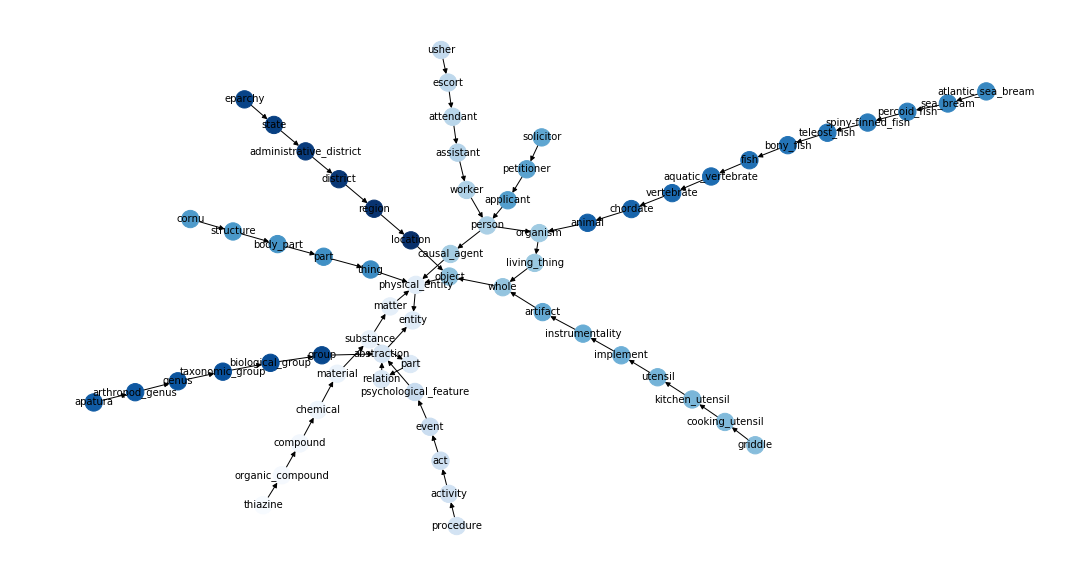
\includegraphics[width=\textwidth]{Wordnet}
	\caption{Wordnet Entities and Relations Graphplot}
\end{figure}

\begin{figure}[H]
   	\centering
    	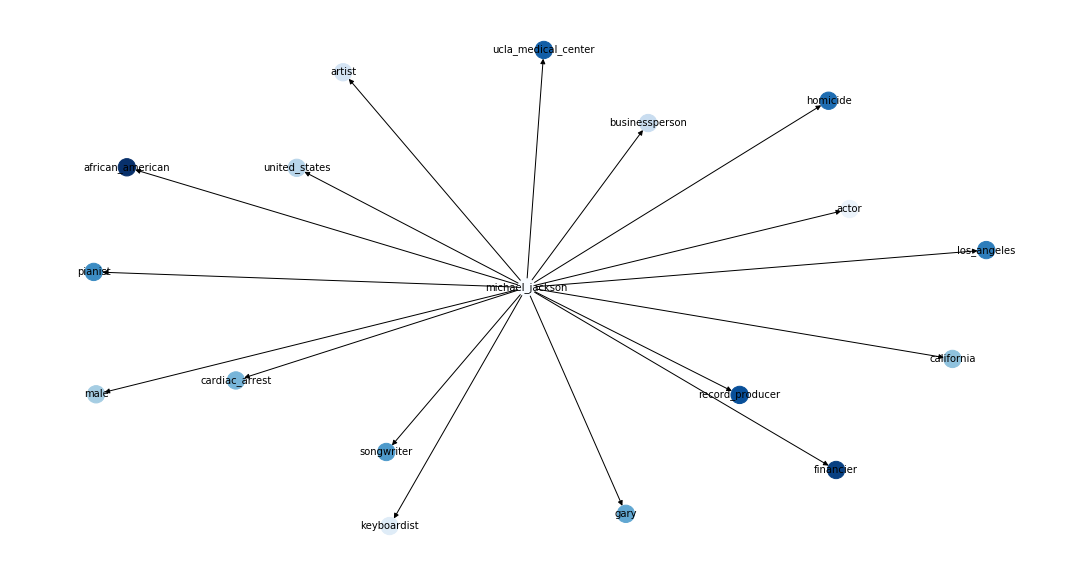
\includegraphics[width=\textwidth]{Freebase}
	\caption{Freebase Entity and Relations Graphplot}
\end{figure}

\noindent We used the TensorFlow framework to implement our updated NTN training algorithm.  This algorithm makes use of the NTN model introduced by (Socher and Chen, et al. 2013) \unskip ~\citep{socher2013reasoning} and re-implemented in TensorFlow by (Doss, LeNail and Liu 2015) \unskip ~\citep{Doss2015}. Pre-trained word vectors are used to initialise entity and relational embeddings during model training. The embedding parameters are adjusted during training to generate latent representations specific to the knowledge domain. Property counts for the respective KGs are presented below:

\bigskip

\begin{figure}[H]
	\parbox{.5\linewidth}{
   		\centering
    		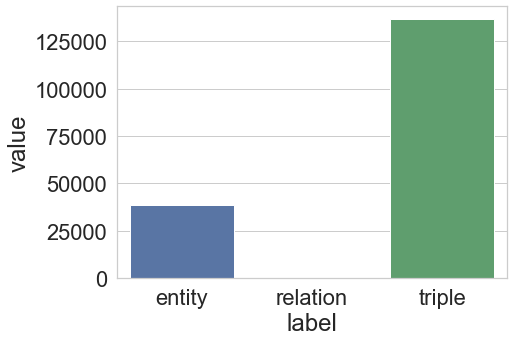
\includegraphics[width=0.45\textwidth]{Wordnet_Counts}
		\caption{Wordnet Property Barplot}
		}
	\hfill
	\parbox{.5\linewidth}{
   		\centering
    		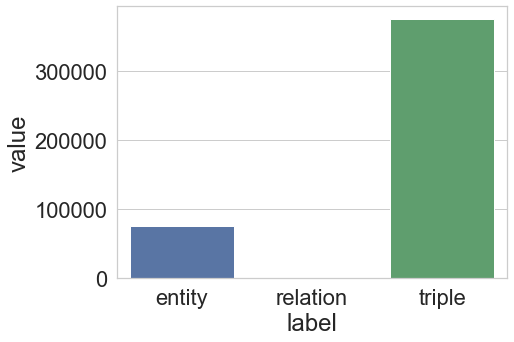
\includegraphics[width=0.45\textwidth]{Freebase_Counts}
		\caption{Freebase Property Barplot}
		}
\end{figure}

\begin{table}[H]
	\parbox{.5\linewidth}{
		\centering
		\begin{tabular}{lllllllllll}
  			\textbf{Property} & \textbf{Count}  \\
  			\hline
  			Entities & 38,696  \\
  			Relations & 11  \\
  			Triples & 136,611  \\
			&
		\end{tabular}
		\caption{Wordnet Property Counts}
		}
	\hfill
	\parbox{.5\linewidth}{
		\centering
		\begin{tabular}{lllllllllll}
  			\textbf{Property} & \textbf{Count}  \\
  			\hline
  			Entities & 75,043   \\
  			Relations & 13  \\
  			Triples & 375,499  \\
			&
		\end{tabular}
		\caption{Freebase Property Counts}
		}
\end{table}

%********************************** %Predicate  **************************************

\noindent Summary statistics of the respective KG RDF formalism are presented below.

\medskip

\begin{figure}[H]
	\parbox{.5\linewidth}{
   		\centering
    		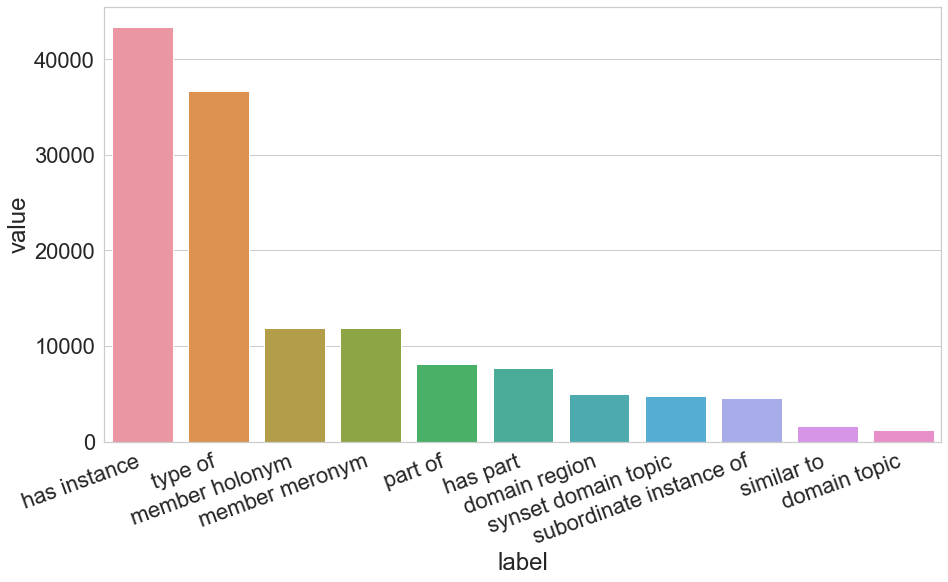
\includegraphics[width=0.45\textwidth, height=0.2\textheight]{Wordnet_Predicate_Counts}
		\caption{Wordnet Predicate Barplot}
		}
	\hfill
	\parbox{.5\linewidth}{
   		\centering
		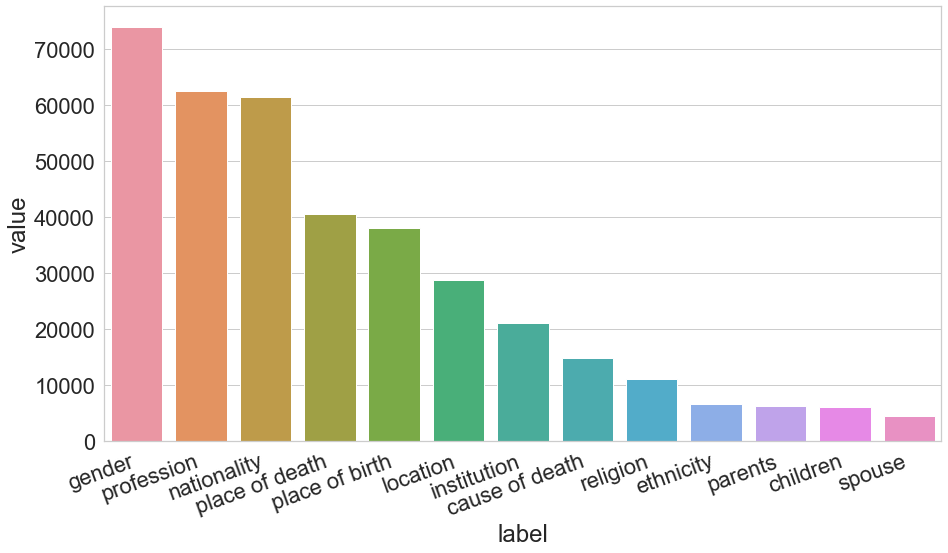
\includegraphics[width=0.45\textwidth, height=0.2\textheight]{Freebase_Predicate_Counts}
		\caption{Freebase Predicate Barplot}
		}
\end{figure}

\begin{table}[H]
	\parbox{.5\linewidth}{
		\centering
		\begin{tabular}{lllllllllll}
  			\textbf{Statistic} & \textbf{Value}  \\
  			\hline
			Count & 11 \\
			Max & 43,312  \\
			Min & 1,229  \\
  			Median & 7,705  \\
  			IQR & 7,257.5  \\
				&
		\end{tabular}
		\caption{Wordnet Predicate Statistics}
		}
	\hfill
	\parbox{.5\linewidth}{
		\centering
		\begin{tabular}{lllllllllll}
  			\textbf{Statistic} & \textbf{Value}  \\
  			\hline
			Count & 13 \\
			Max & 73,897  \\
			Min & 4, 464  \\
  			Median & 21,149  \\
  			IQR & 34,033  \\
				&
		\end{tabular} 
		\caption{Freebase Predicate Statistics}
		}
\end{table}

%********************************** %Subject **************************************

\begin{figure}[H]
	\parbox{.5\linewidth}{
   		\centering
    		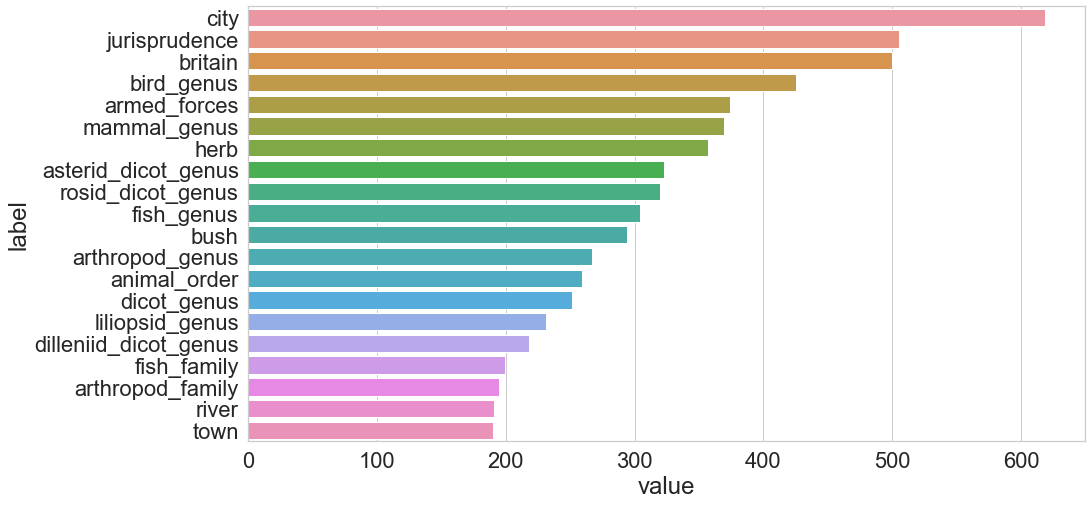
\includegraphics[width=0.45\textwidth, height=0.2\textheight]{Wordnet_Subject_Counts}
		\caption{Wordnet Subject Barplot}
		}
	\hfill
	\parbox{.5\linewidth}{
   		\centering
		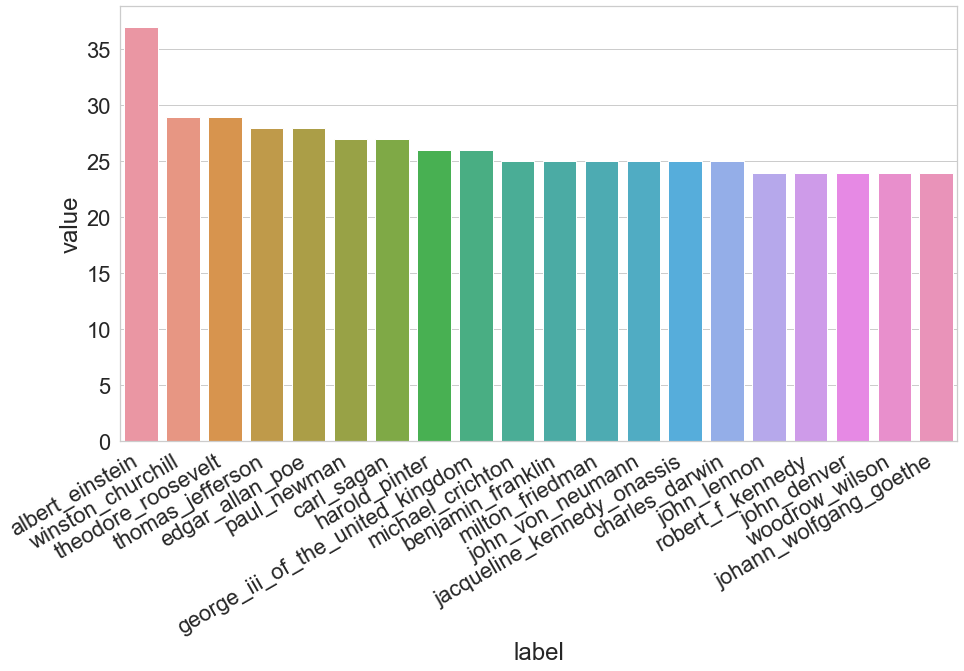
\includegraphics[width=0.45\textwidth, height=0.2\textheight]{Freebase_Subject_Counts}
		\caption{Freebase Subject Barplot}
		}
\end{figure}

\begin{table}[H]
	\parbox{.5\linewidth}{
		\centering
		\begin{tabular}{lllllllllll}
  			\textbf{Statistic} & \textbf{Value}  \\
  			\hline
			Count & 32,720 \\
			Max & 619 \\
			Min & 1 \\
  			Median & 2 \\
  			IQR & 2 \\
				&
		\end{tabular}
		\caption{Wordnet Subject Statistics}
		}
	\hfill
	\parbox{.5\linewidth}{
		\centering
		\begin{tabular}{lllllllllll}
  			\textbf{Statistic} & \textbf{Value}  \\
  			\hline
			Count & 67,393 \\
			Max & 37 \\
			Min & 1 \\
  			Median & 5 \\
  			IQR & 4 \\
				&
		\end{tabular}
		\caption{Freebase Subject Statistics}
		}
\end{table}

%********************************** %Object  **************************************

\begin{figure}[H]
	\parbox{.5\linewidth}{
   		\centering
    		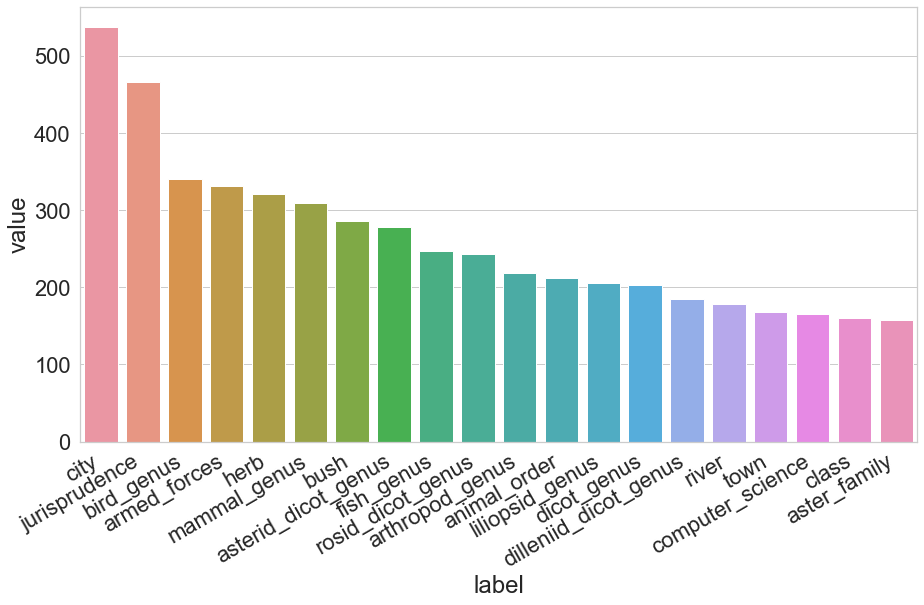
\includegraphics[width=0.45\textwidth, height=0.2\textheight]{Wordnet_Object_Counts}
		\caption{Wordnet Object Barplot}
		}
	\hfill
	\parbox{.5\linewidth}{
   		\centering
		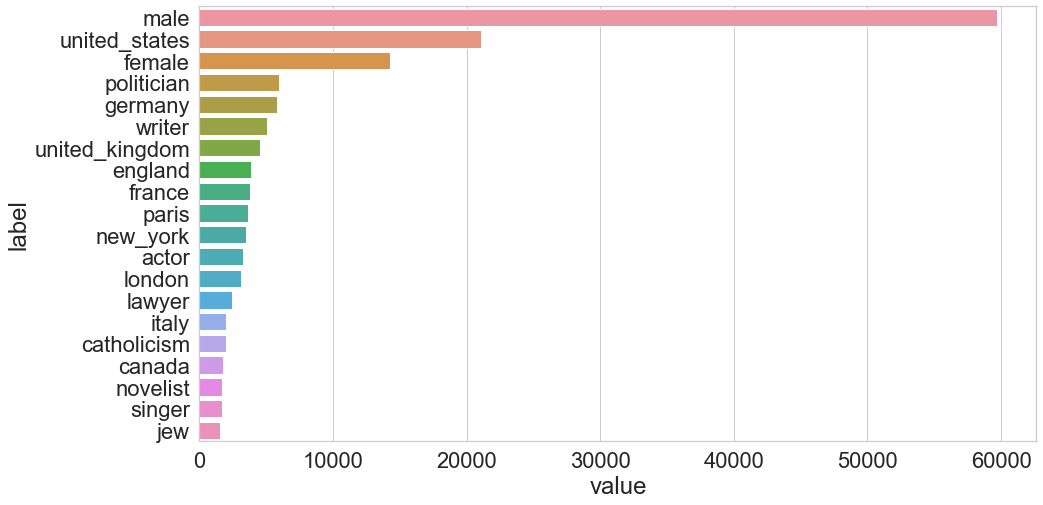
\includegraphics[width=0.45\textwidth, height=0.2\textheight]{Freebase_Object_Counts}
		\caption{Freebase Object Barplot}
		}
\end{figure}


\begin{table}[H]
	\parbox{.5\linewidth}{
		\centering
		\begin{tabular}{lllllllllll}
  			\textbf{Statistic} & \textbf{Value}  \\
  			\hline
			Count & 33,011 \\
			Max & 537 \\
			Min & 1 \\
  			Median & 3 \\
  			IQR & 2 \\
				&
		\end{tabular}
		\caption{Wordnet Object Statistics}
		}
	\hfill
	\parbox{.5\linewidth}{
		\centering
		\begin{tabular}{lllllllllll}
  			\textbf{Statistic} & \textbf{Value}  \\
  			\hline
			Count & 15,342 \\
			Max & 59,663 \\
			Min & 1 \\
  			Median & 3 \\
  			IQR & 6 \\
				&
		\end{tabular}
		\caption{Freebase Object Statistics}
		}
\end{table}

\noindent For Wordnet, it can be seen that relations are skewed toward "has instance" with 43,312 occurrences, and "type of" with 36,659 occurrences. We would expect poor performance from the model for out of sample data containing relations that are not "has instance" or "type of". Freebase relations are somewhat more uniform, however four relations have occurrences under 10,000. We would expect reasonable performance across all relations for this dataset. \par

\noindent Wordnet and Freebae subjects are somewhat uniform, although the median number of occurrences is 2 and 5 respectively, with an IQR of 2 and 4 respectively. These are thus sparse distributions of data points, and the model will need to rely on  similarity of subject features in order to produce sensible inference. Wordnet object occurrences are somewhat uniform whilst Freebase object occurrences are skewed, with a single object, "male" occurring 59,663 times, representing 15,88\% of facts. This is in comparison to a median object occurrence of 3 and an interquartile range of 6. We would expect poor performance from a Freebase link prediction model given this distribution of objects. 


%********************************** %Optimised training algorithm **************************************

\subsection{Optimised training algorithm}

\noindent We update the NTN training algorithm to make use of the Adam optimiser \citep{kingma2014adam}, early stopping \citep{prechelt1998early}, and use random grid search for hyperparameter optimisation \citep{bergstra2012random}. The the model was trained on a MacBook Pro 2015 with 8 cores, 16GB RAM, and 512GB SSD. We evaluate the model by ranking the accuracy scores of the predicted triples for the respective datasets. \par

\noindent \textbf{Code to reproduce} \newline
Updated NTN:  \url{https://github.com/xhosaBoy/deep-knowledge-modelling} \newline
Baseline: \url{https://github.com/xhosaBoy/recursive-neural-tensor-networks}

\noindent \textbf{Link training results.} The cost and accuracy results of NTN model training with the original baseline training algorithm, compared to the optimised training algorithm are presented below.

\begin{figure}[H]
	\parbox{.5\linewidth}{
   		\centering
    		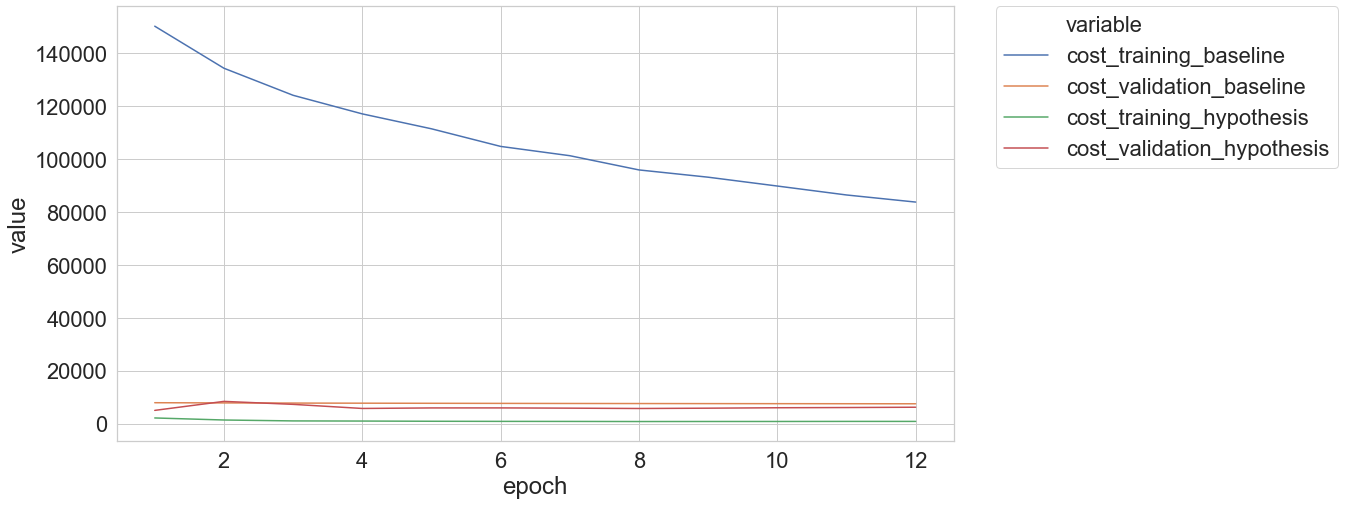
\includegraphics[width=0.45\textwidth, height=0.2\textheight]{Wordnet_Cost_Results_Early_Stopping}
		\caption{Wordnet Cost}
		}
	\hfill
	\parbox{.5\linewidth}{
   		\centering
		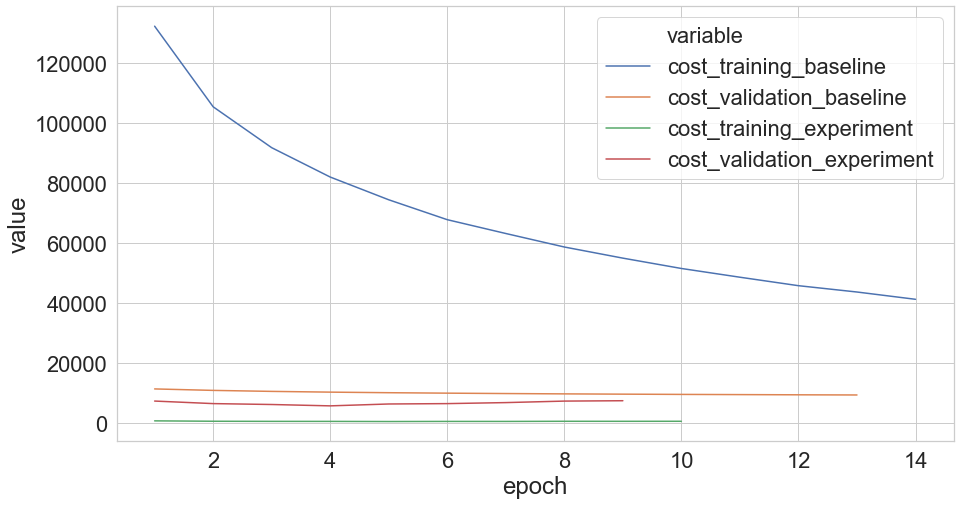
\includegraphics[width=0.45\textwidth, height=0.2\textheight]{Freebase_Cost_Results}
		\caption{Freebase Cost}
		}
\end{figure}

\begin{figure}[H]
	\parbox{.5\linewidth}{
   		\centering
    		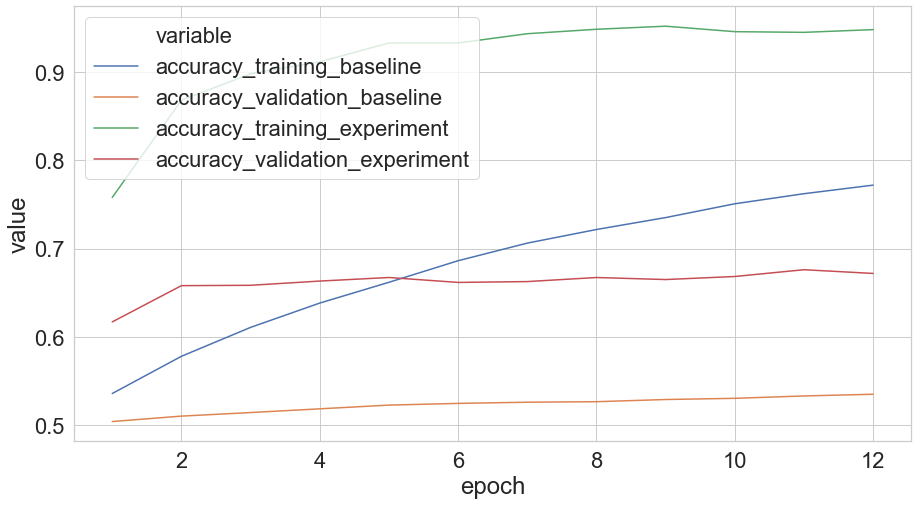
\includegraphics[width=0.45\textwidth, height=0.2\textheight]{Wordnet_Accuracy_Results_Early_Stopping}
		\caption{Wordnet Accuracy}
		}
	\hfill
	\parbox{.5\linewidth}{
   		\centering
		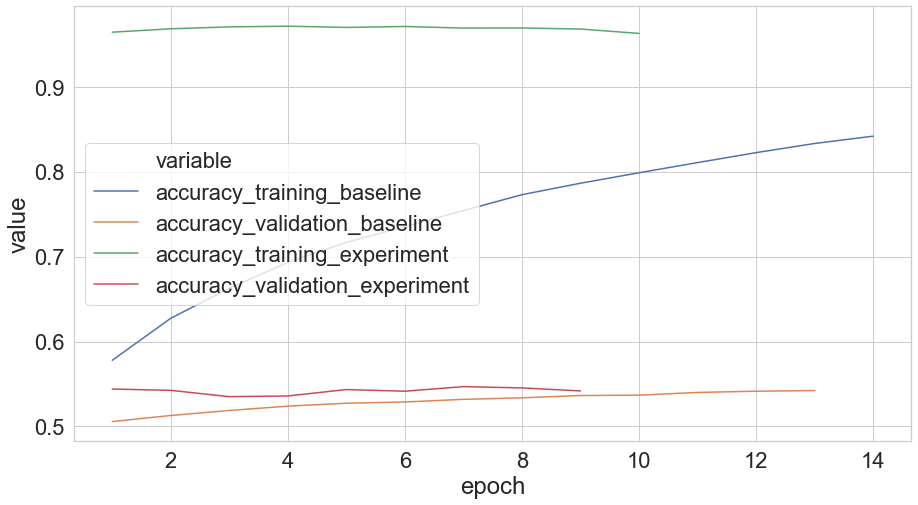
\includegraphics[width=0.45\textwidth, height=0.2\textheight]{Freebase_Accuracy_Results}
		\caption{Freebase Accuracy}
		}
\end{figure}

\begin{table}[H]
	\centering
	\begin{tabular}{lllllllllll}
  		\textbf{Model} & \textbf{Wordnet} & \textbf{Freebbase} & \textbf{Avg} \\
  		\hline
  		Distance Model & .683 & .610 & .647 \\
  		Hadamard Model & .800 & .688 & .744 \\
  		Single Layer Model & .760 & .853 & .807 \\
  		Bilinear Model & \textbf{.841} & \textbf{.877} & \textbf{.859} \\
  		NTN Baseline & .562 & .535 & .549 \\
  		\hline
  		NTN with Optimised Training & .674 & .548 & .611 \\
		&
	\end{tabular}
	\caption{Test cost and accuracy on Wordnet and Freebase KGs}
\end{table}


%********************************** %HypER and Covariate Shift  **************************************

\section{HypER and covariate shift}

\subsection{Baseline training algorithm}
\textbf{Model summary.} HypER is a model that uses relation-specific convolutional filters that are convolved with a subject entity, producing an intermediate entity-relational representation. This representation is then flattened and passed through a nonlinearity before the dot product taken with an object entity. This computation generates a relational score between the two entities, which is then passed through a logistic sigmoid to compute a probability of relational plausibility. \par

\noindent \textbf{Binary cross entropy loss.} The binary cross entropy loss is used to train HypER. Like the NTN model, the input consists of an subject-predicate pair, and an object is presented as a target to complete the triple. A relational score is generated for each sample and passed through through a logistic sigmoid. Loss is generated by comparing the produced likelihood with the expected likelihood, 0 or 1. The sum of all losses is aggregated and back propagated through the network for parameter update. \par

\noindent \textbf{Experimental setup.} We use the following link prediction benchmark datasets: WN18 \citep{bordes2013translating} is a subset of Wordnet, a database containing lexical relations between words. The knowledge graph contains 40,943 entities and 18 relations. FB15k \citep{bordes2013translating} is a subset of Freebase, a large database of facts about the real world. FB15k contains 14,951 entities and 1,345 relations. Visualisations of the respective knowledge graphs are presented below.

\bigskip

\begin{figure}[H]
   	\centering
    	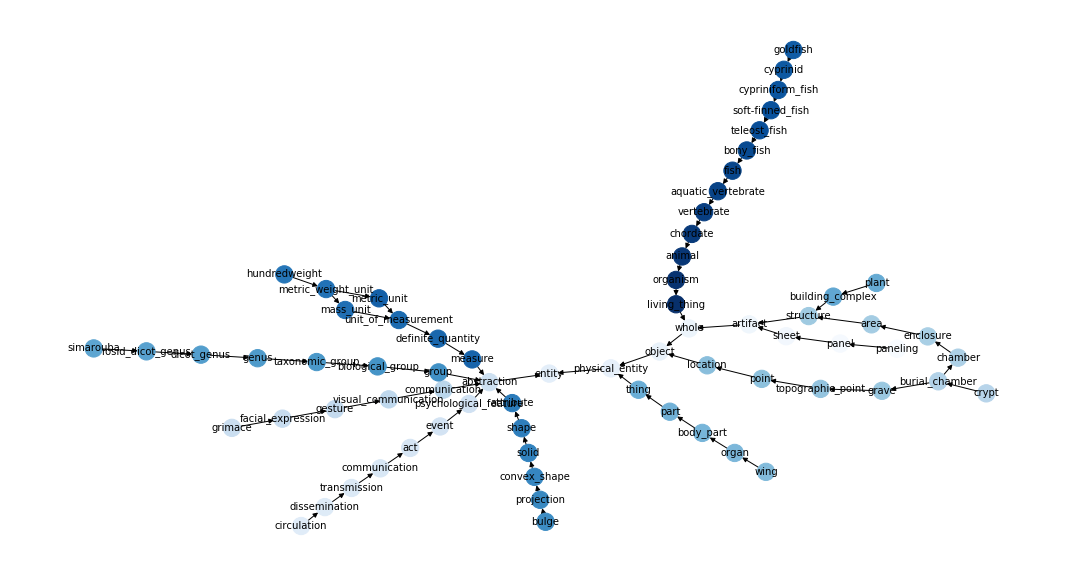
\includegraphics[width=\textwidth]{WN18_Graph}
	\caption{WN18 Entities and Relations Graphplot}
\end{figure}

\begin{figure}[H]
   	\centering
    	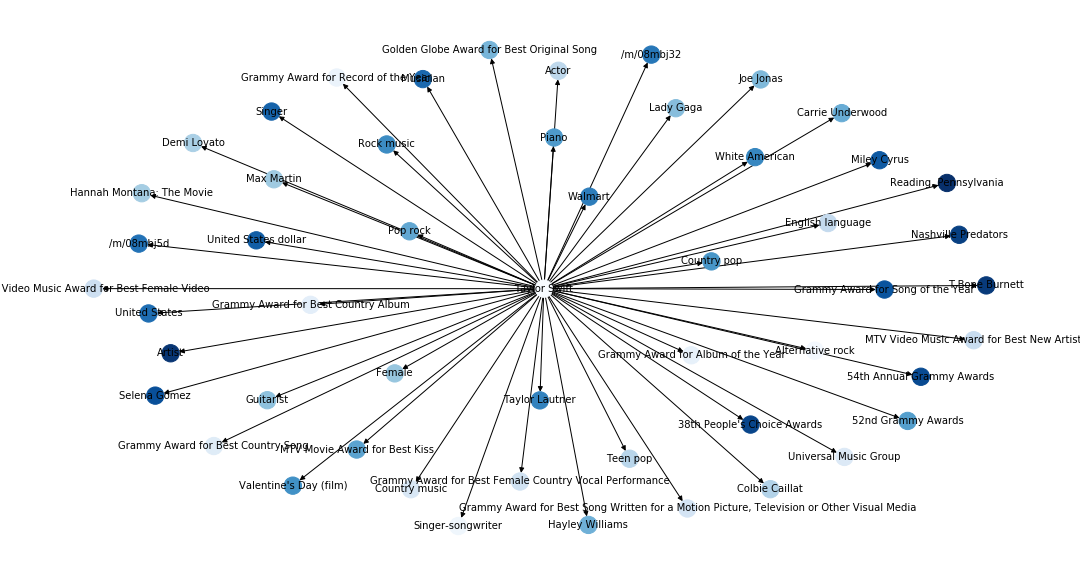
\includegraphics[width=\textwidth]{FB15k_Graph}
	\caption{FB15k Entity and Relations Graphplot}
\end{figure}

\noindent We used the Pytorch framework to develop our model. This model is built on top of the HypER model introduced by Balaˇzevi´c, et al. ~\citep{balazevic2019hypernetwork}. Randomly initialised entity and relational embeddings are used to initialise model training. These embeddings are dynamically adjusted during the training process to generate latent representations specific to the knowledge domain. Property counts for the respective knowledge graphs are presented below.

\bigskip

\begin{figure}[H]
	\parbox{.5\linewidth}{
   		\centering
    		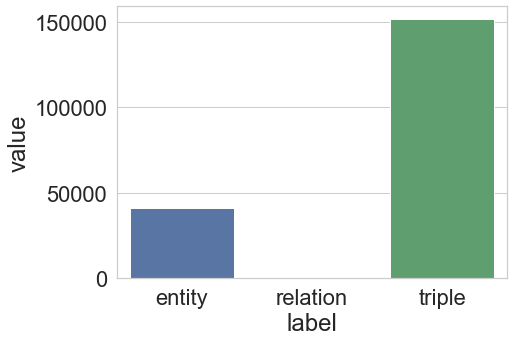
\includegraphics[width=0.45\textwidth]{WN18_Counts}
		\caption{WN18 Property Barplot}
		}
	\hfill
	\parbox{.5\linewidth}{
   		\centering
    		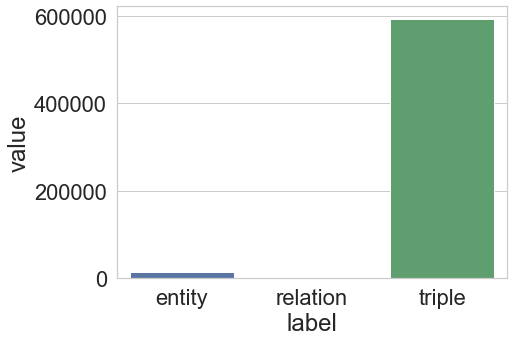
\includegraphics[width=0.45\textwidth]{FB15k_Counts}
		\caption{FB15k Property Barplot}
		}
\end{figure}

\begin{table}[H]
	\parbox{.5\linewidth}{
		\centering
		\begin{tabular}{lllllllllll}
  			\textbf{Property} & \textbf{Count}  \\
  			\hline
  			Entities & 40,943  \\
  			Relations & 18  \\
  			Triples & 151,442 \\
			&
		\end{tabular}
		\caption{WN18 Property Counts}
		}
	\hfill
	\parbox{.5\linewidth}{
		\centering
		\begin{tabular}{lllllllllll}
  			\textbf{Property} & \textbf{Count}  \\
  			\hline
  			Entities & 14,951   \\
  			Relations & 1,345  \\
  			Triples & 592,213  \\
			&
		\end{tabular}
		\caption{FB15k Property Counts}
		}
\end{table}

%********************************** %Predicate  **************************************

\noindent Summary statistics of the respective KG RDF formalism are presented below.

\begin{figure}[H]
	\parbox{.5\linewidth}{
   		\centering
    		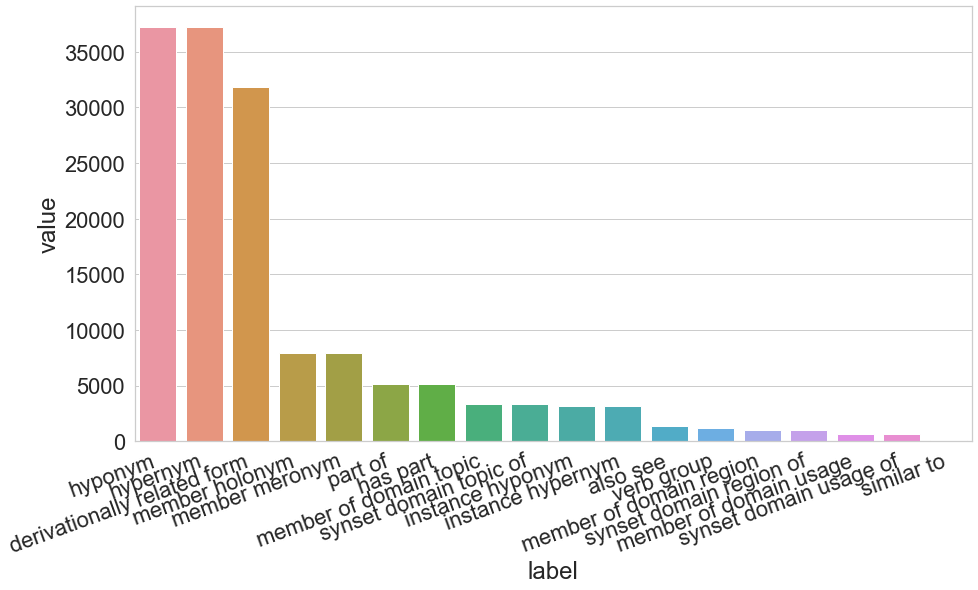
\includegraphics[width=0.45\textwidth, height=0.2\textheight]{WN18_Predicate_Counts}
		\caption{WN18 Predicate Barplot}
		}
	\hfill
	\parbox{.5\linewidth}{
   		\centering
		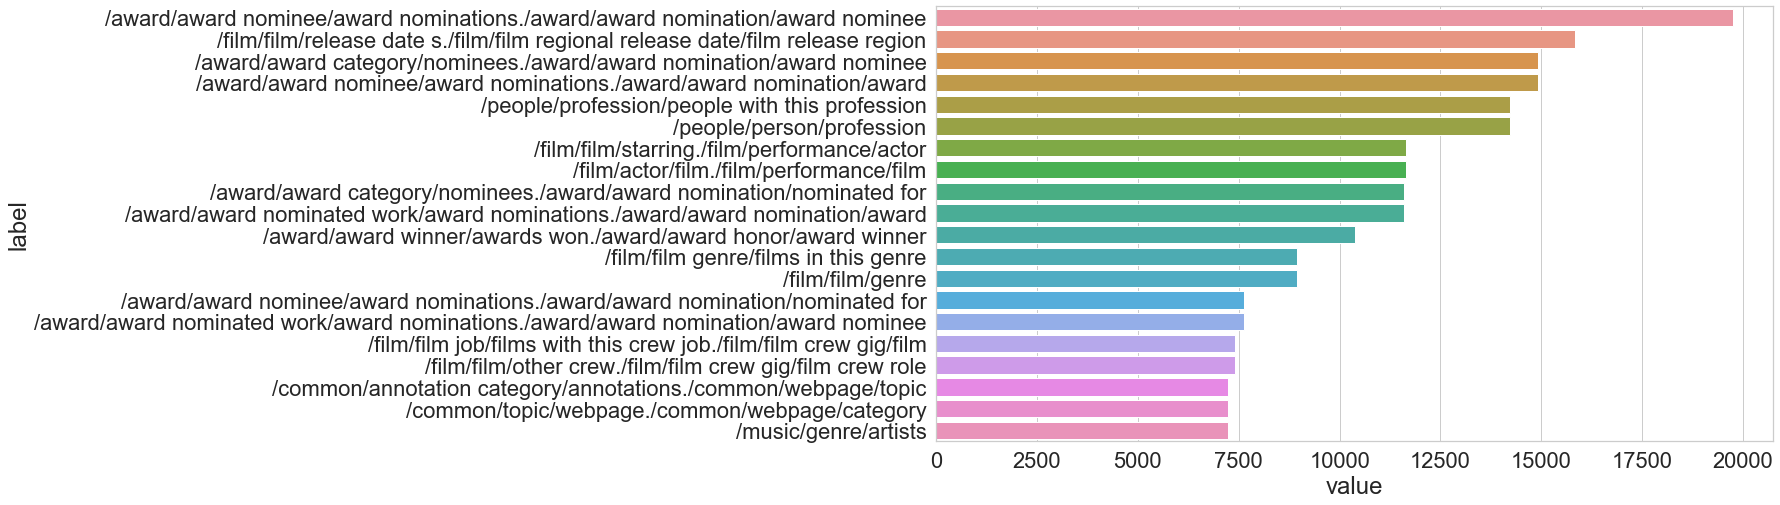
\includegraphics[width=0.45\textwidth, height=0.2\textheight]{FB15k_Predicate_Counts}
		\caption{FB15k Predicate Barplot}
		}
\end{figure}

\begin{table}[H]
	\parbox{.5\linewidth}{
		\centering
		\begin{tabular}{lllllllllll}
  			\textbf{Statistic} & \textbf{Value}  \\
  			\hline
			Count & 18 \\
			Max & 37,221  \\
			Min & 86 \\
  			Median & 3,242.5  \\
  			IQR & 6,190.75  \\
			&
		\end{tabular}
		\caption{WN18 Predicate Statistics}
		}
	\hfill
	\parbox{.5\linewidth}{
		\centering
		\begin{tabular}{lllllllllll}
  			\textbf{Statistic} & \textbf{Value}  \\
  			\hline
			Count & 1,345 \\
			Max & 19,764  \\
			Min & 1  \\
  			Median & 26  \\
  			IQR & 166  \\
			&
		\end{tabular}
		\caption{FB15k Predicate Statistics}
		}
\end{table}

%********************************** %Subject **************************************

\begin{figure}[H]
	\parbox{.5\linewidth}{
   		\centering
    		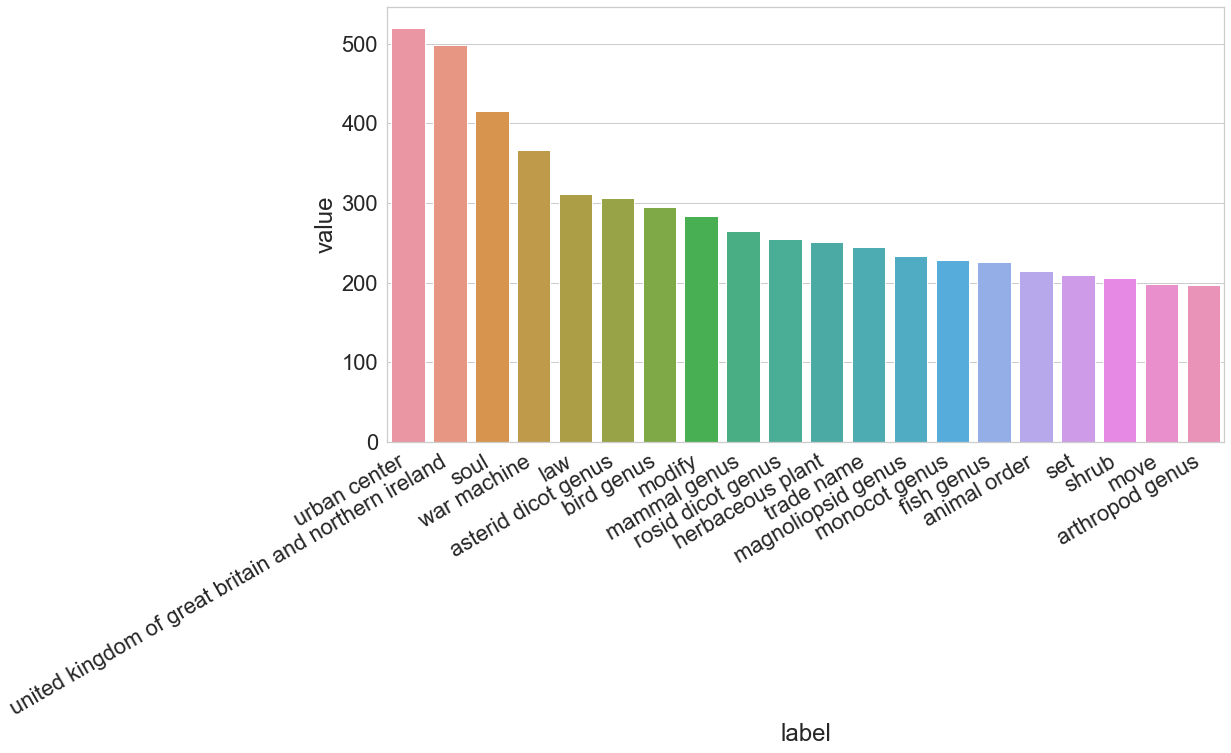
\includegraphics[width=0.45\textwidth, height=0.2\textheight]{WN18_Subject_Counts}
		\caption{WN18 Subject Barplot}
		}
	\hfill
	\parbox{.5\linewidth}{
   		\centering
		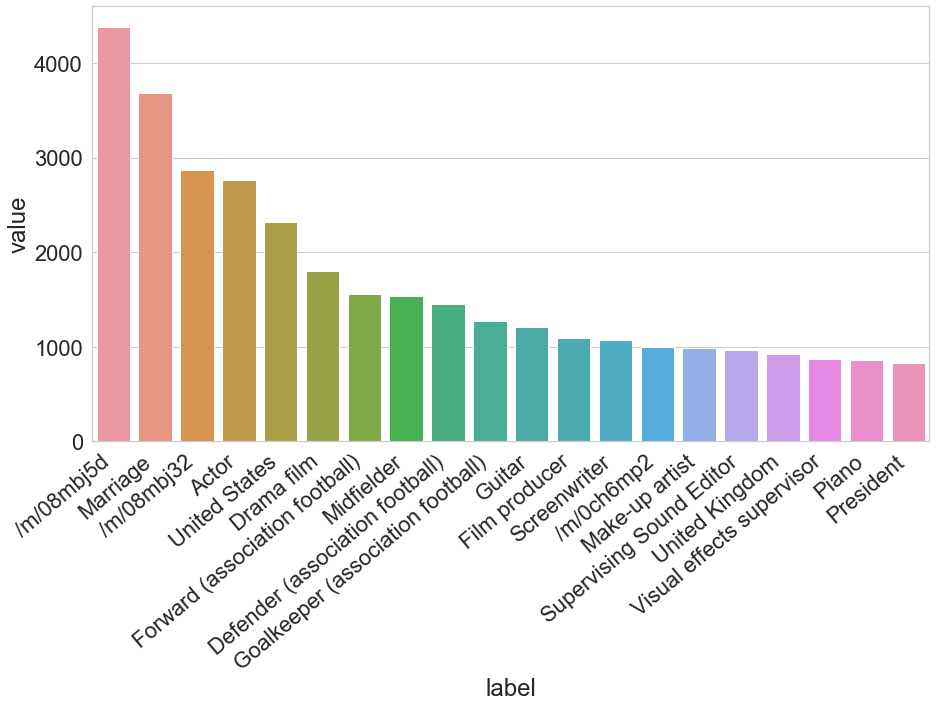
\includegraphics[width=0.45\textwidth, height=0.2\textheight]{FB15k_Subject_Counts}
		\caption{FB15k Subject Barplot}
		}
\end{figure}

\begin{table}[H]
	\parbox{.5\linewidth}{
		\centering
		\begin{tabular}{lllllllllll}
  			\textbf{Statistic} & \textbf{Value}  \\
  			\hline
			Count & 32,544 \\
			Max & 520 \\
			Min & 1 \\
  			Median & 3 \\
  			IQR & 2 \\
			&
		\end{tabular}
		\caption{WN18 Subject Statistics}
		}
	\hfill
	\parbox{.5\linewidth}{
		\centering
		\begin{tabular}{lllllllllll}
  			\textbf{Statistic} & \textbf{Value}  \\
  			\hline
			Count &14,865 \\
			Max & 4,381 \\
			Min & 1 \\
  			Median & 27 \\
  			IQR & 32 \\
			&
		\end{tabular}
		\caption{FB15k Subject Statistics}
		}
\end{table}

%********************************** %Object  **************************************

\begin{figure}[H]
	\parbox{.5\linewidth}{
   		\centering
    		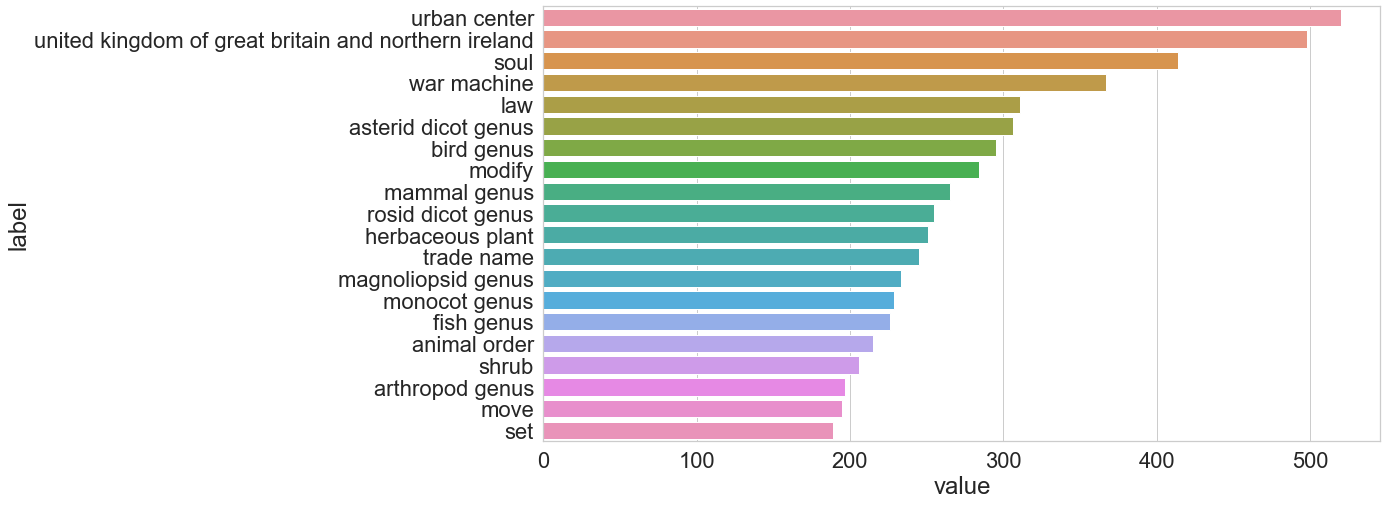
\includegraphics[width=0.45\textwidth, height=0.2\textheight]{WN18_Object_Counts}
		\caption{WN18 Object Barplot}
		}
	\hfill
	\parbox{.5\linewidth}{
   		\centering
		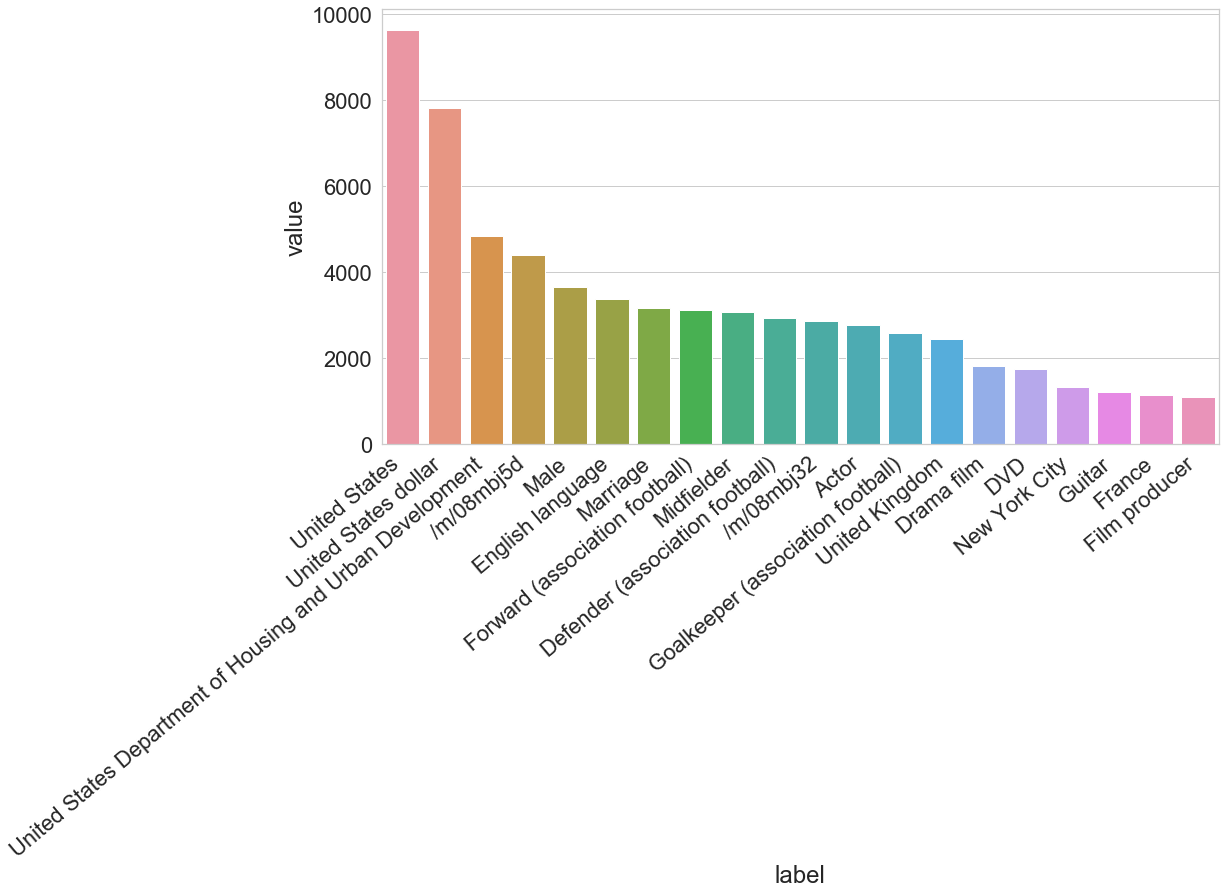
\includegraphics[width=0.45\textwidth, height=0.2\textheight]{FB15k_Object_Counts}
		\caption{FB15k Object Barplot}
		}
\end{figure}

\begin{table}[H]
	\parbox{.5\linewidth}{
		\centering
		\begin{tabular}{lllllllllll}
  			\textbf{Statistic} & \textbf{Value}  \\
  			\hline
			Count & 32,543 \\
			Max & 520 \\
			Min & 1 \\
  			Median & 3 \\
  			IQR & 2 \\
			&
		\end{tabular}
		\caption{WN18 Object Statistics}
		}
	\hfill
	\parbox{.5\linewidth}{
		\centering
		\begin{tabular}{lllllllllll}
  			\textbf{Statistic} & \textbf{Value}  \\
  			\hline
			Count & 14,930 \\
			Max & 9,645 \\
			Min & 1 \\
  			Median & 23 \\
  			IQR & 30 \\
			&
		\end{tabular}
		\caption{FB15k Object Statistics}
		}
\end{table}

\noindent For WN18, it can be seen that relations are skewed toward the relations "hyponym",  "hypernym", and "derivationally related from", with a maximum of 37,221 occurrences. FB15k relations are somewhat more uniform. We would expect reasonable performance across all relations for this knowledge graph. WN18 and FB15k subjects are somewhat uniform aside from a small number of high occurrences entities, with the median number of occurrences is 3 and 27 respectively, and with an IQR of 2 and 32 respectively. WN18 object occurrences are somewhat uniform. FB15k object occurrences are skewed, with the "United States" partaking in the highest number of facts. This is in comparison to a median object occurrence of 3 and an interquartile range of 23.


%********************************** %HypER+  **************************************

\subsection{HypER+}
HypER relational filter inputs generated by a hypernetwork suffer from distribution shift during training, covariate shift. We compensate for this covariate shift by introducing batch normalisation for relational inputs, and introduce HypER+. The the model was trained on Google Cloud Platform, on a N1 series instance with  8 CPU cores, 30GB RAM, 512GB SSD and a Nvidia Tesla P100 GPU. We evaluate the model using standard link prediction benchmarks. \par

\noindent \textbf{Code to reproduce} \newline
HypER+: \url{https://github.com/xhosaBoy/HypER-Regularised-Relations} \newline
Baseline: \url{https://github.com/xhosaBoy/HypER-baseline}

\noindent \textbf{Link prediction results.} The link prediction benchmark results of the HypER+ model, compared against other link prediction models, are presented below.

%********************************** %Cost  **************************************

\bigskip

\begin{figure}[H]
	\parbox{.5\linewidth}{
   		\centering
    		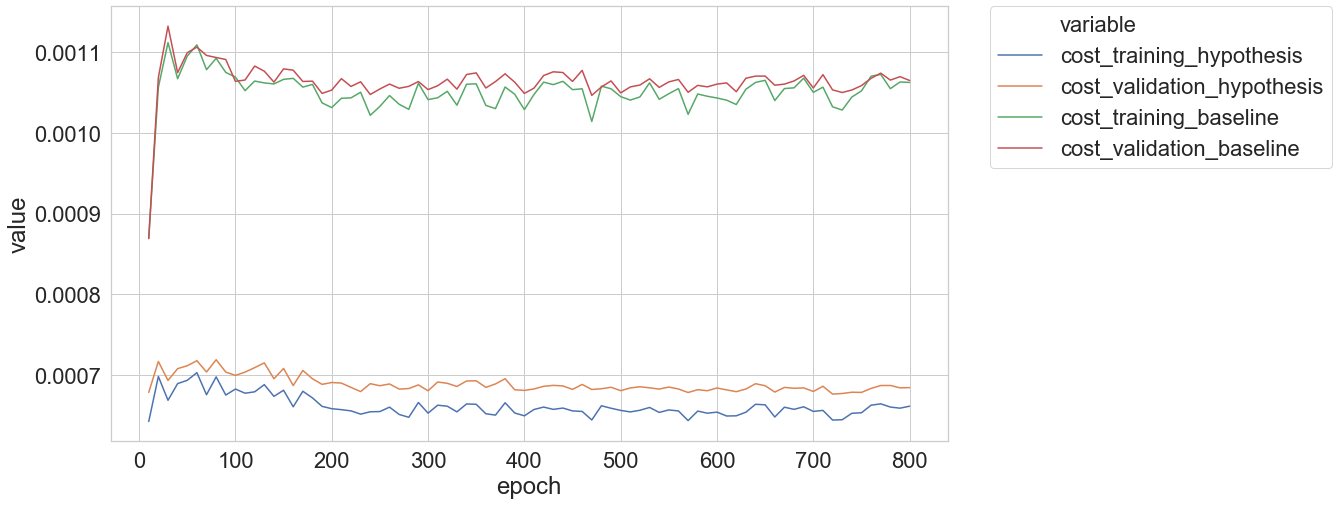
\includegraphics[width=0.45\textwidth, height=0.2\textheight]{WN18_Cost_Results}
		\caption{WN18 Cost}
		}
	\hfill
	\parbox{.5\linewidth}{
   		\centering
		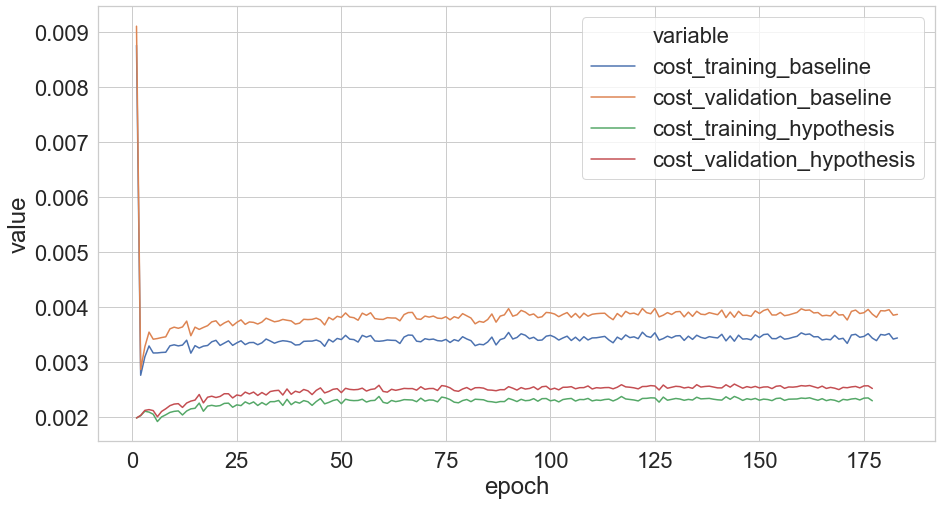
\includegraphics[width=0.45\textwidth, height=0.2\textheight]{FB15k_Cost_Results}
		\caption{FB15k Cost}
		}
\end{figure}


%********************************** %Hits@10  **************************************

\begin{figure}[H]
	\parbox{.5\linewidth}{
   		\centering
    		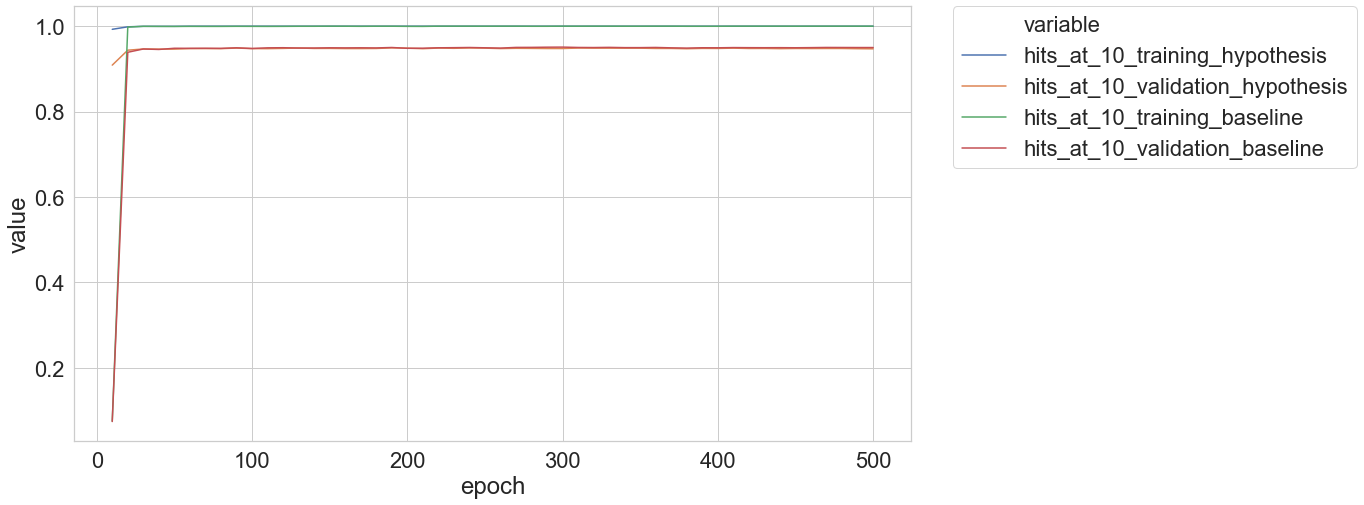
\includegraphics[width=0.45\textwidth, height=0.2\textheight]{WN18_hits_at_10_Results}
		\caption{WN18 Hits@10}
		}
	\hfill
	\parbox{.5\linewidth}{
   		\centering
		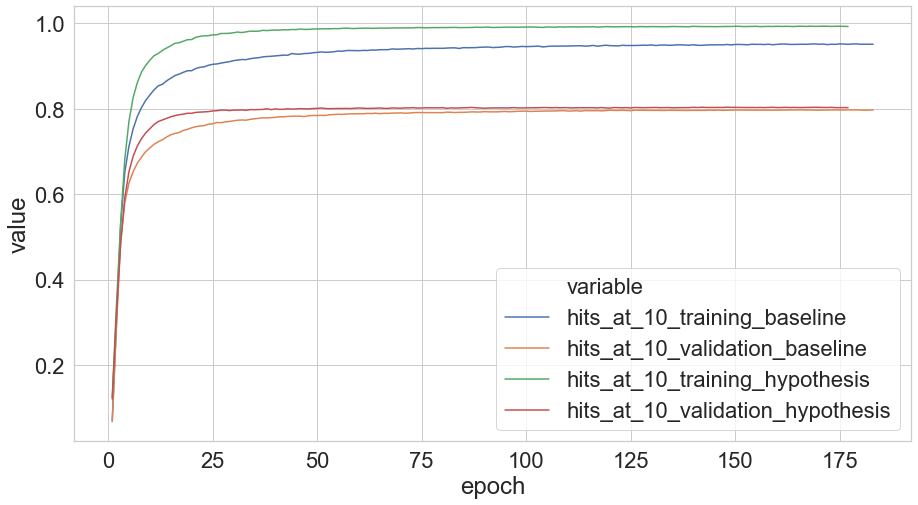
\includegraphics[width=0.45\textwidth, height=0.2\textheight]{FB15k_hits_at_10_Results}
		\caption{FB15k Hits@10}
		}
\end{figure}

%********************************** %Hits@3  **************************************

\begin{figure}[H]
	\parbox{.5\linewidth}{
   		\centering
    		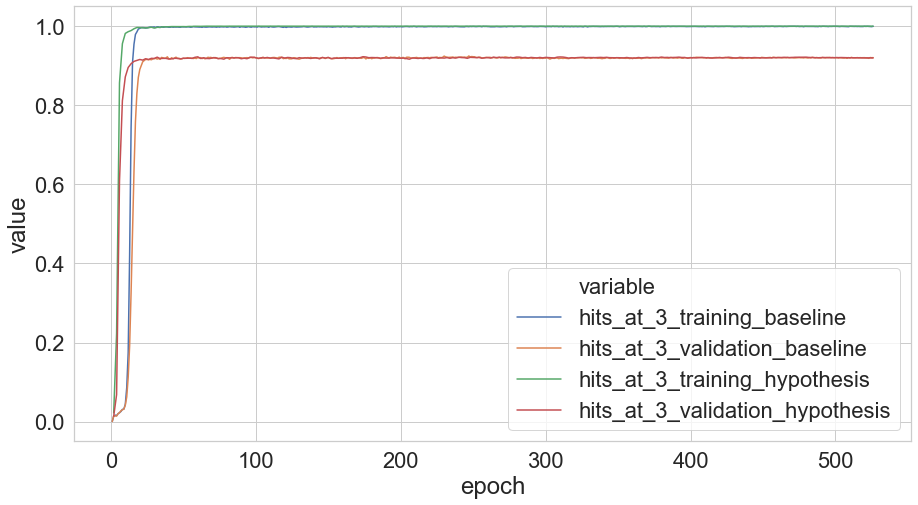
\includegraphics[width=0.45\textwidth, height=0.2\textheight]{WN18_hits_at_3_Results}
		\caption{WN18 Hits@3}
		}
	\hfill
	\parbox{.5\linewidth}{
   		\centering
		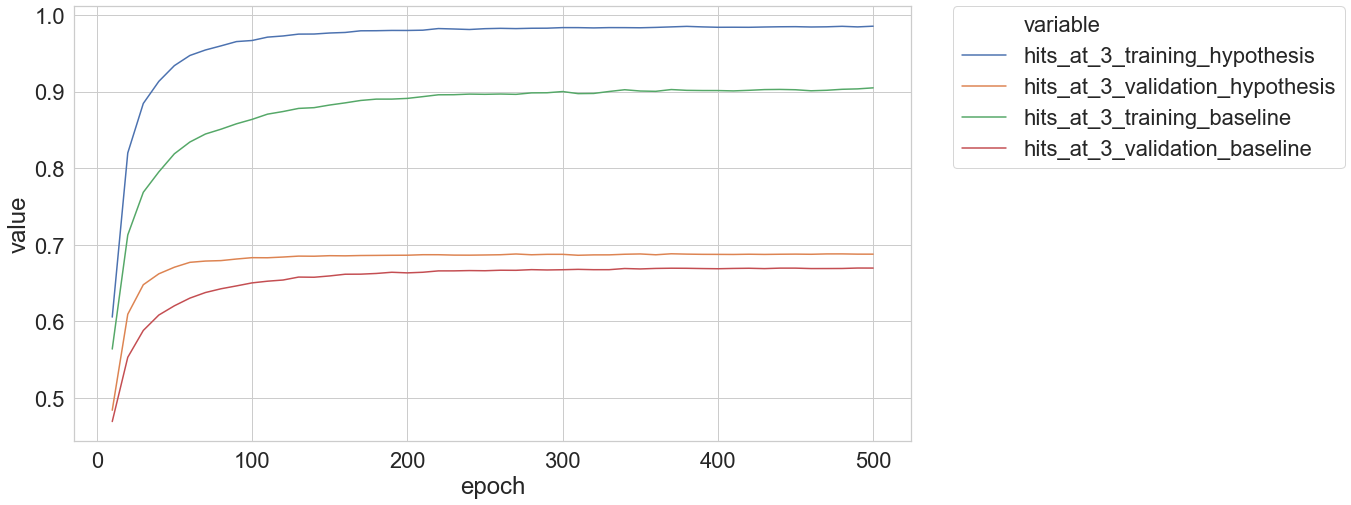
\includegraphics[width=0.45\textwidth, height=0.2\textheight]{FB15k_hits_at_3_Results}
		\caption{FB15k Hits@3}
		}
\end{figure}

%********************************** %Hits@1  **************************************

\begin{figure}[H]
	\parbox{.5\linewidth}{
   		\centering
    		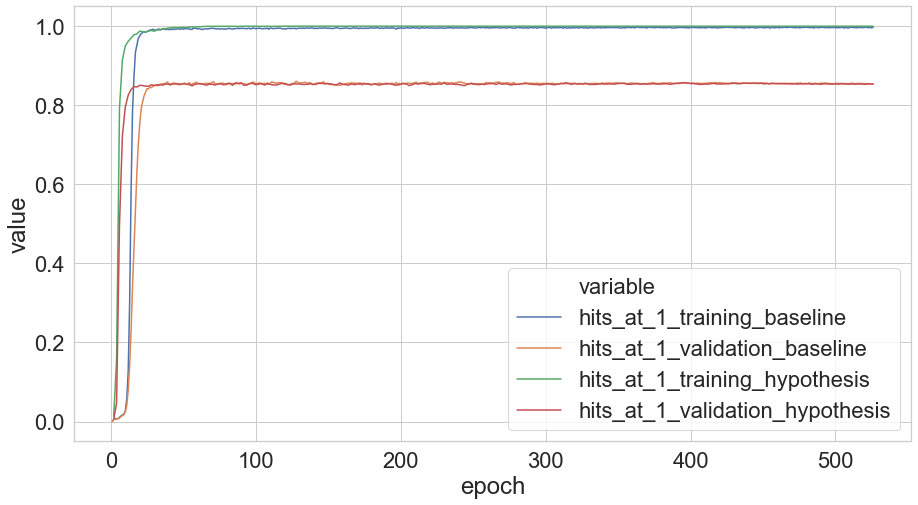
\includegraphics[width=0.45\textwidth, height=0.2\textheight]{WN18_hits_at_1_Results}
		\caption{WN18 Hits@1}
		}
	\hfill
	\parbox{.5\linewidth}{
   		\centering
		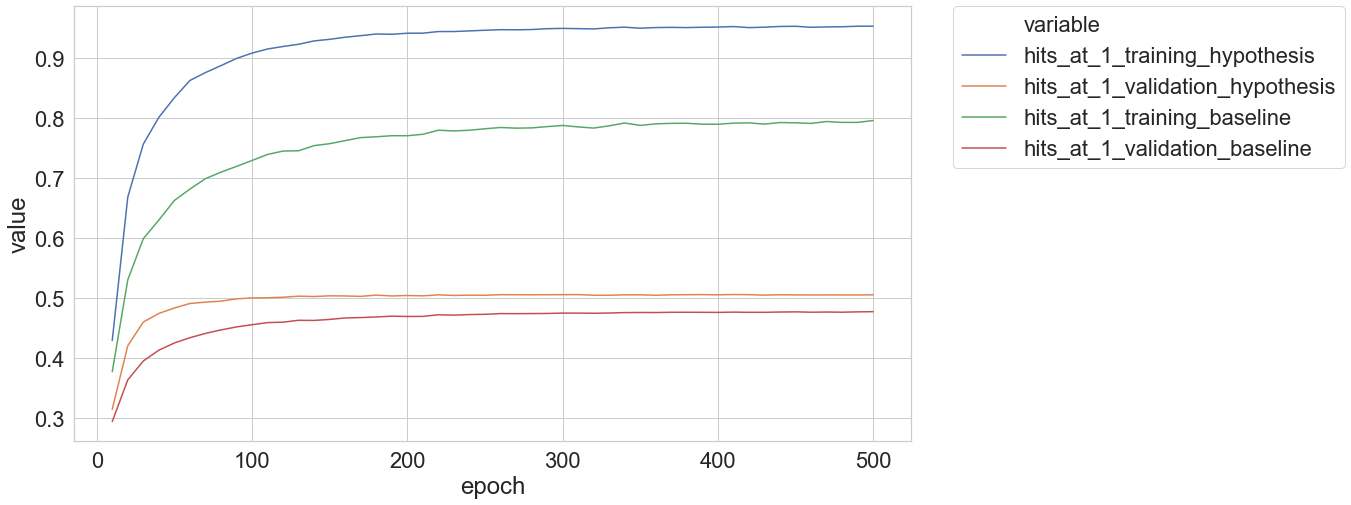
\includegraphics[width=0.45\textwidth, height=0.2\textheight]{FB15k_hits_at_1_Results}
		\caption{FB15k Hits@1}
		}
\end{figure}

%********************************** %Mean rank **************************************

\begin{figure}[H]
	\parbox{.5\linewidth}{
   		\centering
    		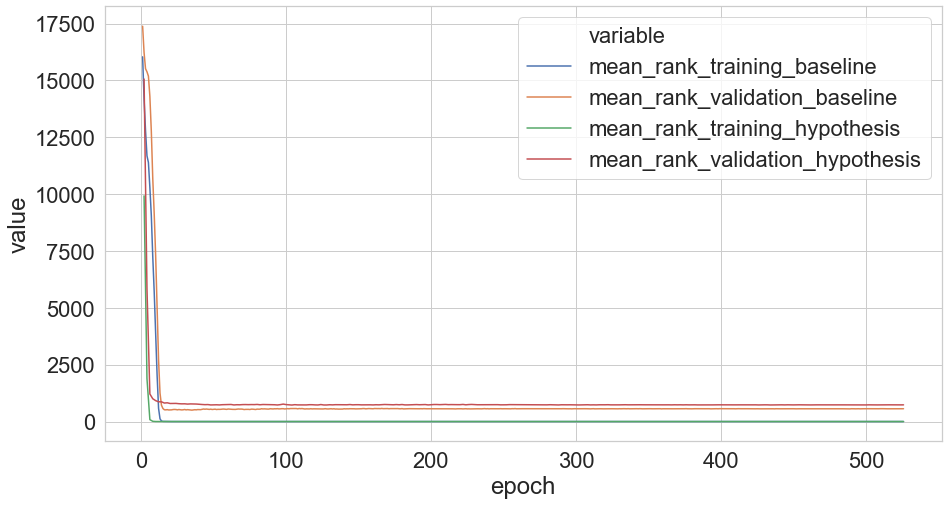
\includegraphics[width=0.45\textwidth, height=0.2\textheight]{WN18_mean_rank_Results}
		\caption{WN18 Mean Rank}
		}
	\hfill
	\parbox{.5\linewidth}{
   		\centering
		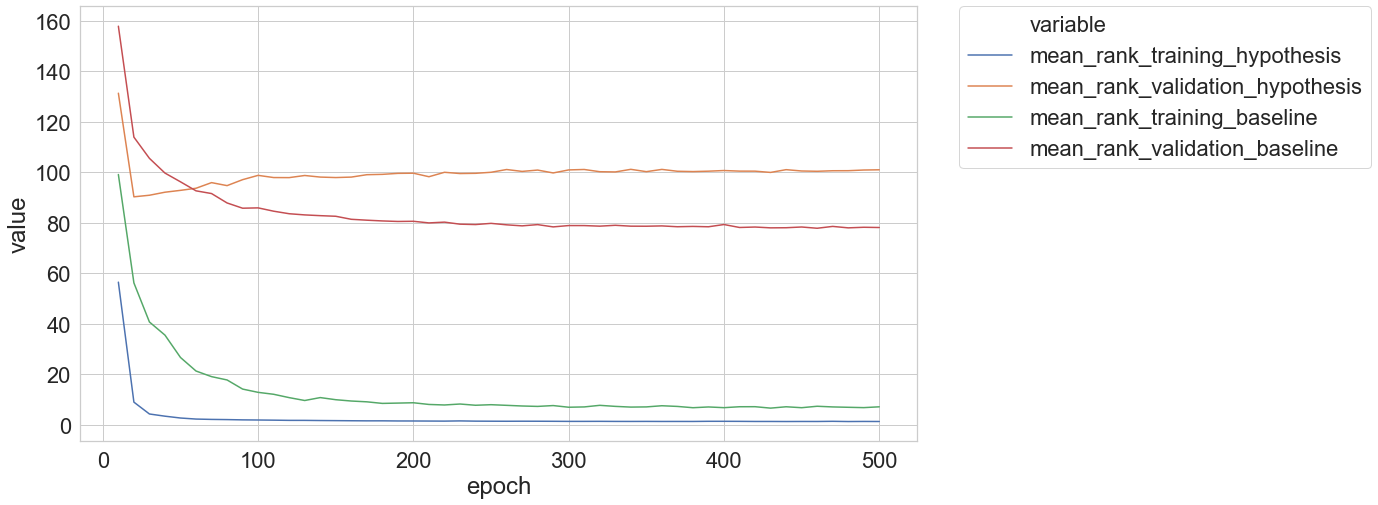
\includegraphics[width=0.45\textwidth, height=0.2\textheight]{FB15k_mean_rank_Results}
		\caption{FB15k Mean Rank}
		}
\end{figure}

%********************************** %Mean reciprocal rank **************************************

\begin{figure}[H]
	\parbox{.5\linewidth}{
   		\centering
    		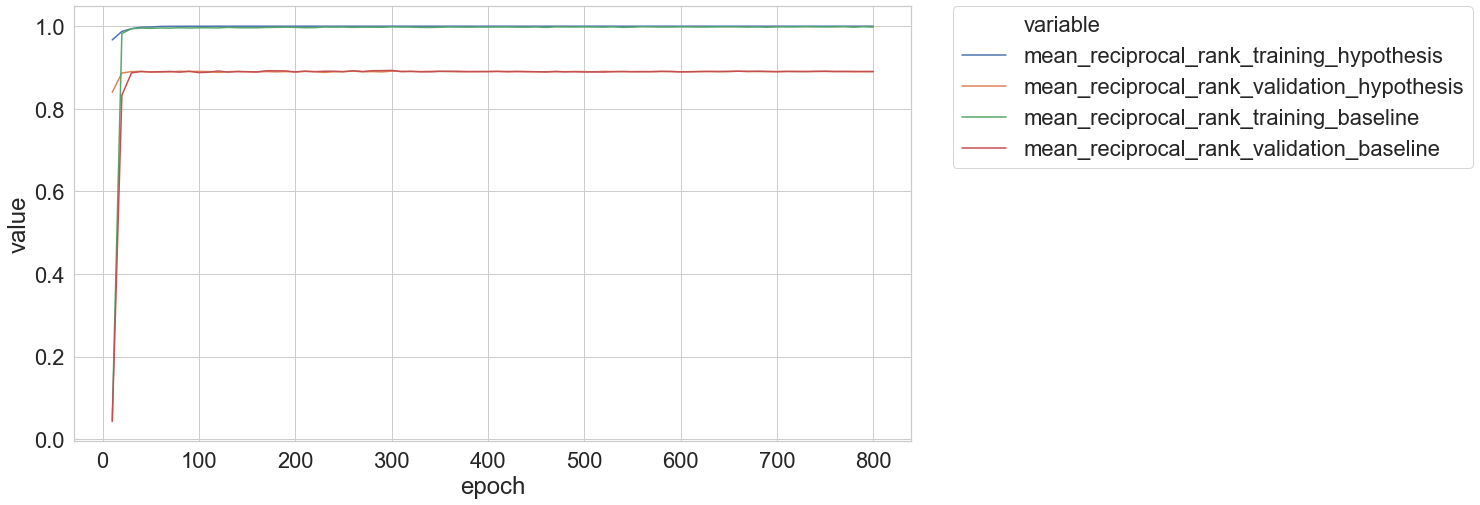
\includegraphics[width=0.45\textwidth, height=0.2\textheight]{WN18_mean_reciprocal_rank_Results}
		\caption{WN18 Mean Reciprocal Rank}
		}
	\hfill
	\parbox{.5\linewidth}{
   		\centering
		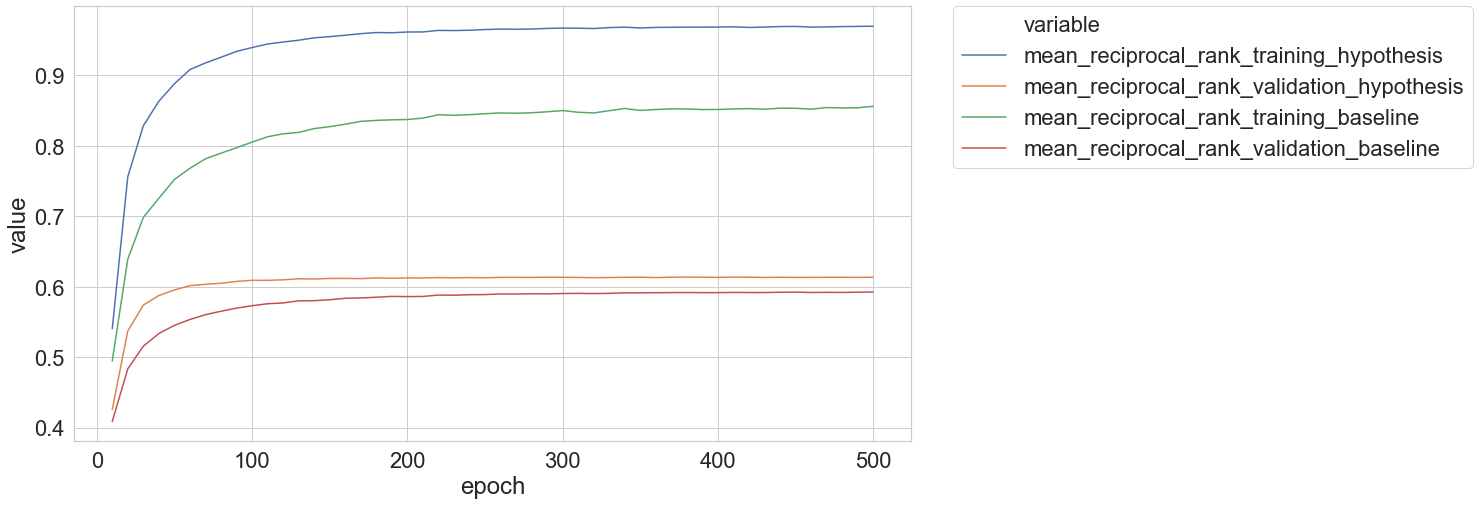
\includegraphics[width=0.45\textwidth, height=0.2\textheight]{FB15k_mean_reciprocal_rank_Results}
		\caption{FB15k Mean Reciprocal Rank}
		}
\end{figure}

%********************************** %Test results **************************************

\begin{table}[H]
	\parbox{.5\linewidth}{
		\centering
		\resizebox{0.5\columnwidth}{!}{%
		\begin{tabular}{lllllllllll}
  			\textbf{Model} & \textbf{H@10} & \textbf{H@3} & \textbf{H@1} & \textbf{MR} & \textbf{MRR} \\
  			\hline
  			TransE (Bordes et al. 2013) & .892 & - & - & \textbf{251} & - \\
  			DistMult (Yang et al. 2015) & .936 & .914 & .728 & 902 & .822 \\
  			ComplEx (Trouillon et al. 2016) & .947 & .936 & .936 & - & .941 \\
  			ANALOGY (Liu, Wu, and Yang 2017) & .947 & .944 & .939 & - & .942 \\
  			Neural LP (Yang, Yang, and Cohen 2017) & .945 & - & - & - & .940 \\
			R-GCN (Schlichtkrull et al. 2018) & \textbf{.964} & .929 & .697 & - & .819 \\
			TorusE (Ebisu and Ichise 2018) & .954 & .950 & .943 & - & .947 \\
			ConvE (Dettmers et al. 2018) & .956 & .946 & .935 & 374 & .943 \\
			HypER (Bala\v{z}evi\'c et al. 2019) & .958 & \textbf{.955} & \text{.947} & 431 & \textbf{.951} \\
  			\hline
  			HypER+ (ours) & .957 & .954 & .946 & 565 & .950 \\
		\end{tabular}
		}
		\caption{Test results on WN18}
	}
	\hfill
	\parbox{.5\linewidth}{
		\centering
		\resizebox{0.5\columnwidth}{!}{
		\begin{tabular}{lllllllllll}
  			\textbf{Model} & \textbf{H@10} & \textbf{H@3} & \textbf{H@1} & \textbf{MR} & \textbf{MRR} \\
  			\hline
  			TransE (Bordes et al. 2013) & .471 & - & - & 125 & - \\
  			DistMult (Yang et al. 2015) & .824 & .733 & .546 & 97 & .654 \\
  			ComplEx (Trouillon et al. 2016) & .840 & .759 & .599 & - & .692 \\
  			ANALOGY (Liu, Wu, and Yang 2017) & .854 & .785 & .646 & - & .725 \\
  			Neural LP (Yang, Yang, and Cohen 2017) & .837 & - & - & - & .760 \\
			R-GCN (Schlichtkrull et al. 2018) & .842 & .760 & .601 & - & .696 \\
			TorusE (Ebisu and Ichise 2018) & .832 & .771 & .674 & - & .733\\
			ConvE (Dettmers et al. 2018) & .831 & .723 & .558 & 51 & .657 \\
			HypER (Bala\v{z}evi\'c et al. 2019) & .885 & .829 & .734 & \textbf{44} & .790 \\
  			\hline
  			HypER+ (ours) & \textbf{.894} & \textbf{.856} & \textbf{.790} & 79 & \textbf{.829} \\
		\end{tabular}
		}
		\caption{Test results on FB15k}
	}
\end{table}

%********************************** %T-SNE **************************************

\begin{figure}[H]
	\parbox{.5\linewidth}{
   		\centering
    		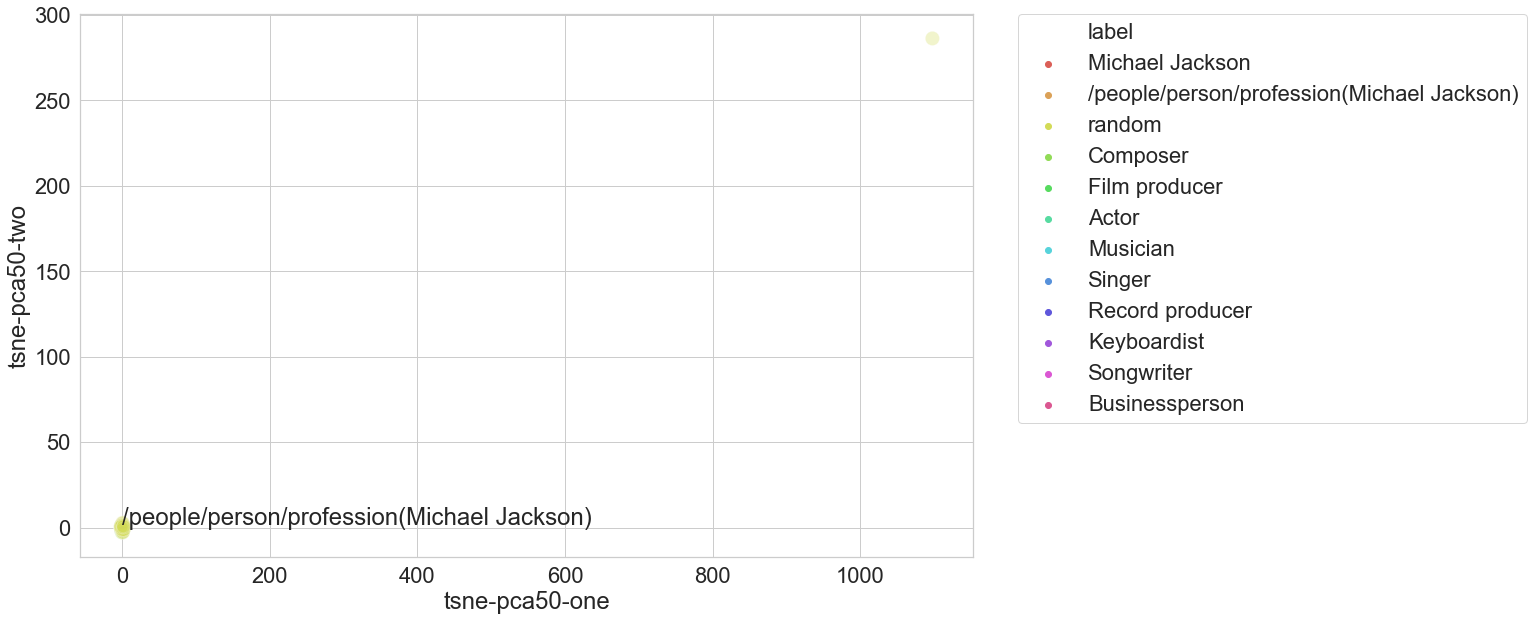
\includegraphics[width=0.4\textwidth, height=0.2\textheight]{t_sne_train_profession}
		\captionsetup{justification=centering}
		\caption{FB15k T-SNE: Michael Jackson Profession Facts, Pre-Training}
		}
	\hfill
	\parbox{.5\linewidth}{
   		\centering
		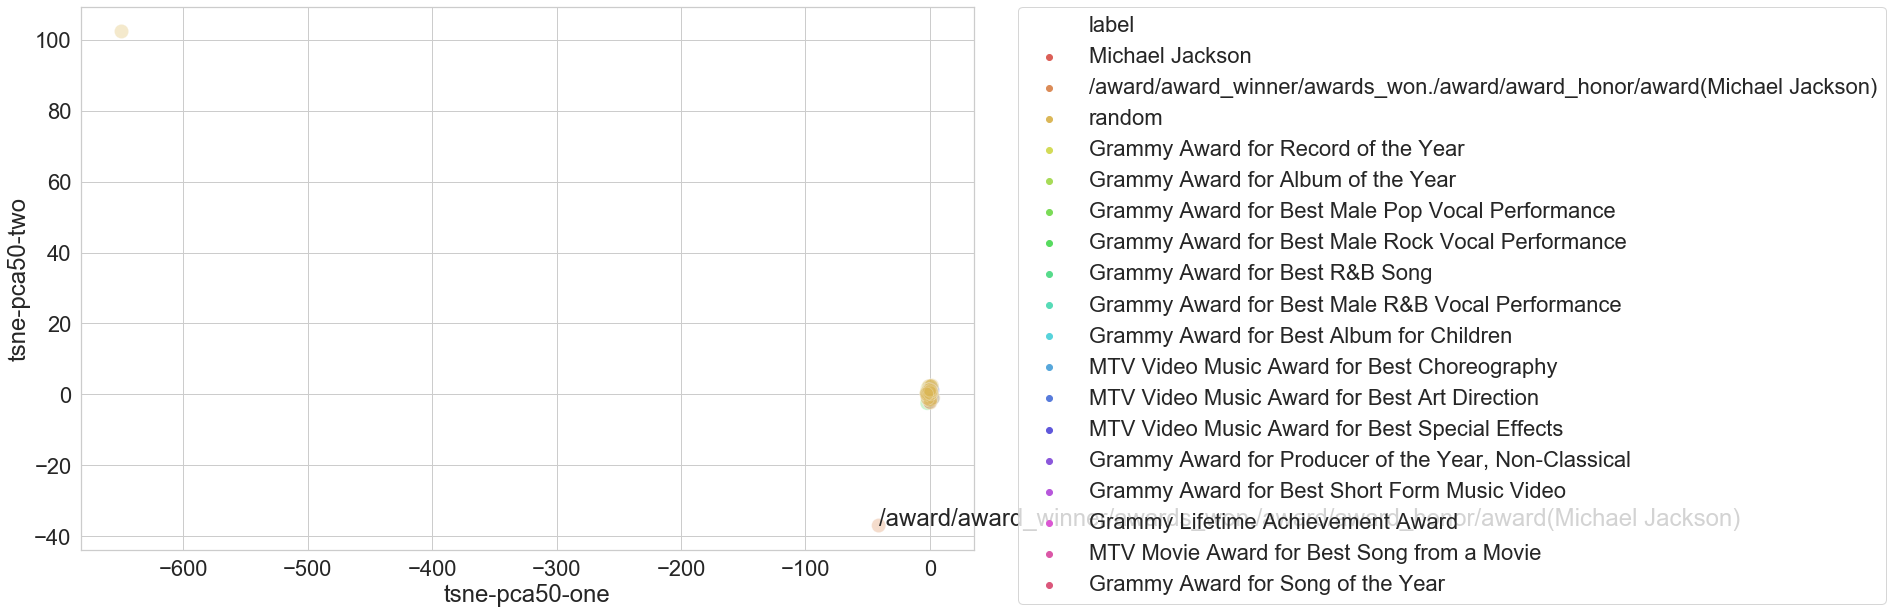
\includegraphics[width=0.5\textwidth, height=0.2\textheight]{t_sne_train_award}
		\captionsetup{justification=centering}
		\caption{FB15k T-SNE: Michael Jackson Award Facts, Pre-Training}
		}
\end{figure}

\begin{figure}[H]
	\parbox{.5\linewidth}{
   		\centering
    		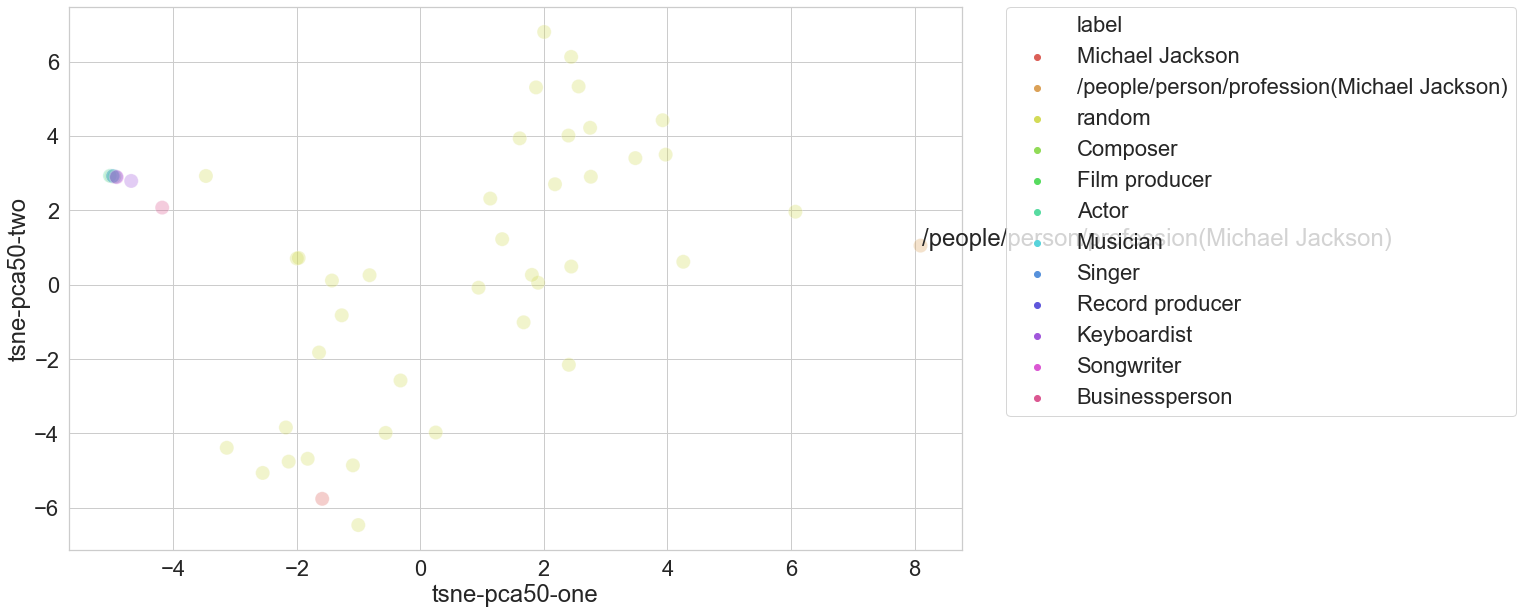
\includegraphics[width=0.4\textwidth, height=0.2\textheight]{t_sne_test_profession}
		\captionsetup{justification=centering}
		\caption{FB15k T-SNE: Michael Jackson Profession Facts, Post-Training}
		}
	\hfill
	\parbox{.5\linewidth}{
   		\centering
		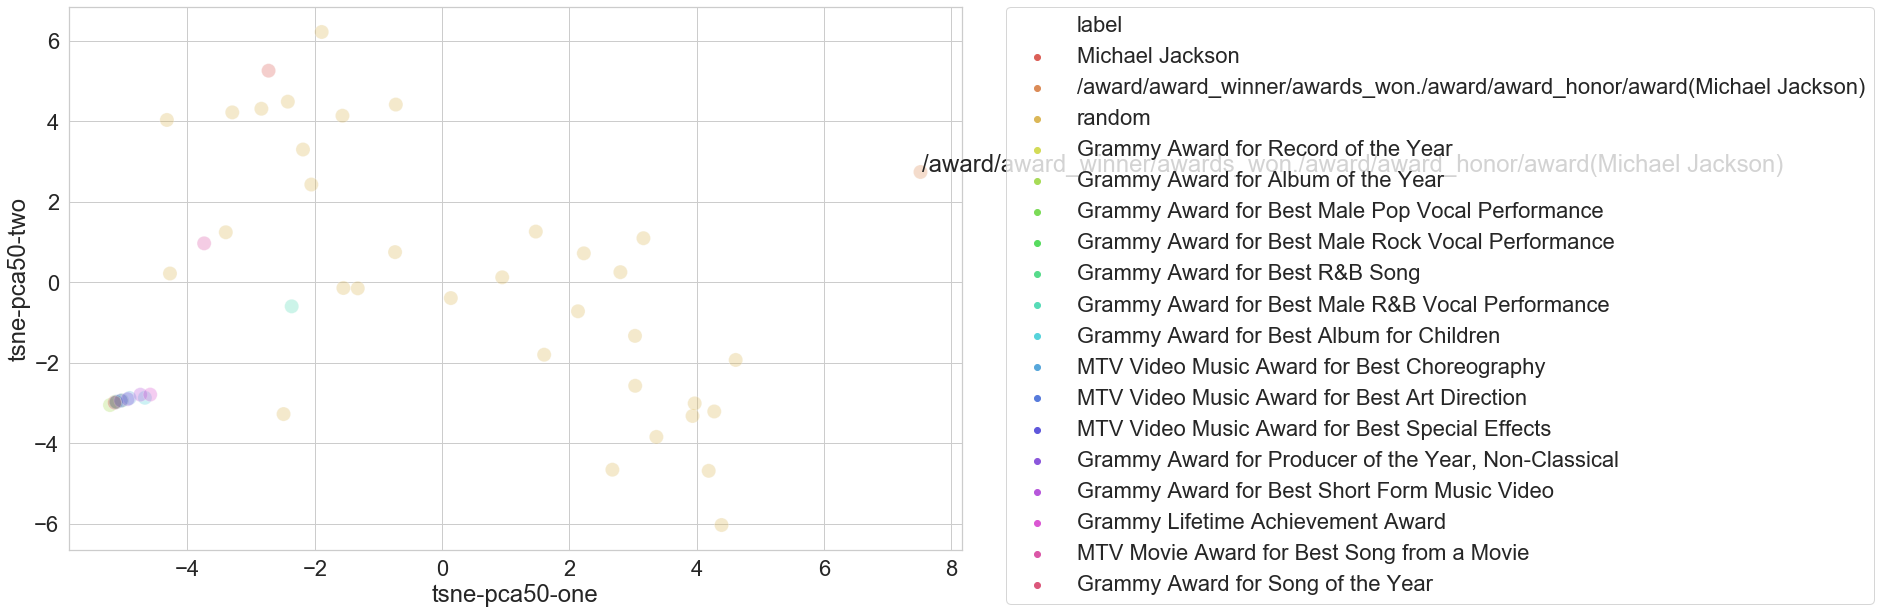
\includegraphics[width=0.5\textwidth, height=0.2\textheight]{t_sne_test_award}
		\captionsetup{justification=centering}
		\caption{FB15k T-SNE: Michael Jackson Award Facts, Post-Training}
		}
\end{figure}

\newpage


%********************************** %HypER+ with Pre-Trained Word Embeddings  **************************************

\section{HypER+ with pre-trained word vectors}

\textbf{Model summary.} We extend HypER+ to make use of pre-trained GloVe word vectors. This model replaces Xavier initailised entity and relation embeddings with aggregated GloVe embeddings. 
HypER+ is also trained using the binary cross entropy loss. \par

\noindent \textbf{Experimental setup.} We use the following benchmark datasets: WN18RR is a subset of WN18, created by Dettmers et al. by removing the inverse relations from WN18. WN18RR contains 40,943 entities and 11 relations. FB15k-237 - was created by Toutanova et al., noting that the validation and test sets of FB15k and WN18 contain the inverse of many relations present in the training set, making it easy for simple models to do well. FB15k-237 is a subset of FB15k with the inverse relations removed. It contains 14,541 entities and 237 relations. Visualisations of the respective knowledge graphs are presented below. 

\begin{figure}[H]
   	\centering
    	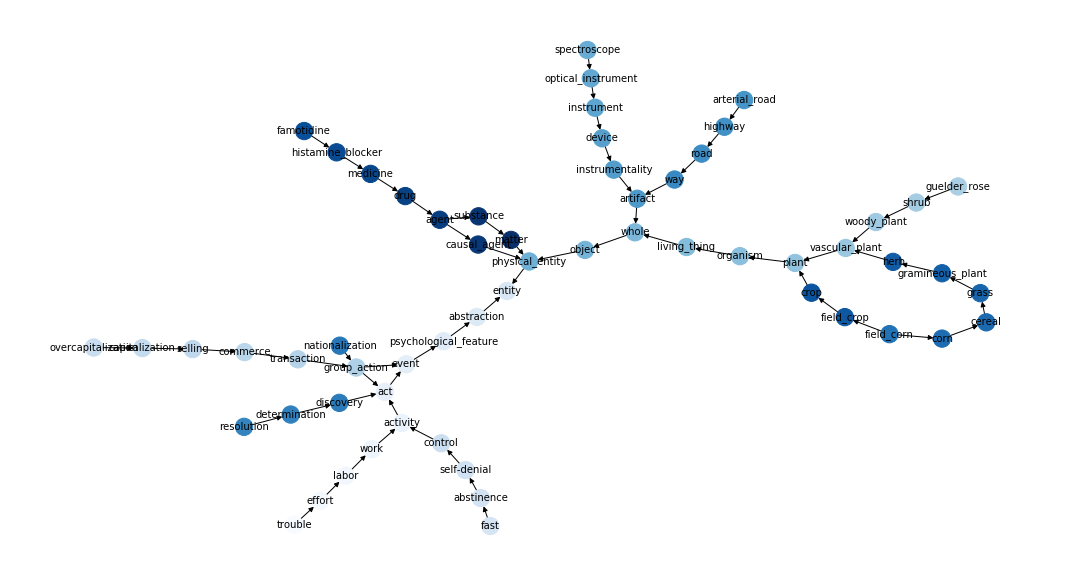
\includegraphics[width=\textwidth]{WN18RR_Graph}
	\caption{WN18RR Entities and Relations Graphplot}
\end{figure}

\begin{figure}[H]
   	\centering
    	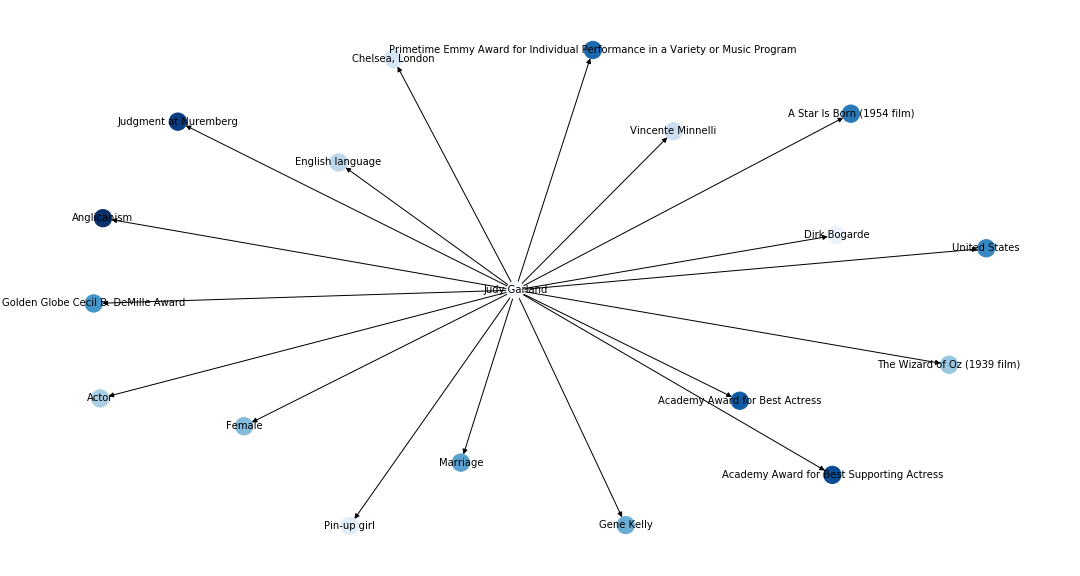
\includegraphics[width=\textwidth]{FB15k-237_Graph}
	\caption{FB15k-237 Entity and Relations Graphplot}
\end{figure}

\noindent We used the Pytorch framework to develop our model. This model is built on top of the HypER+ model introduced by Magangane and Brink.  Glove pre-trained word vectors are used to initialise entity and relational embeddings for model training. These embeddings are dynamically adjusted during the training process to generate latent representations specific to the knowledge domain. Property counts for the respective knowledge graphs are presented below. \par

\begin{figure}[H]
	\parbox{.5\linewidth}{
   		\centering
    		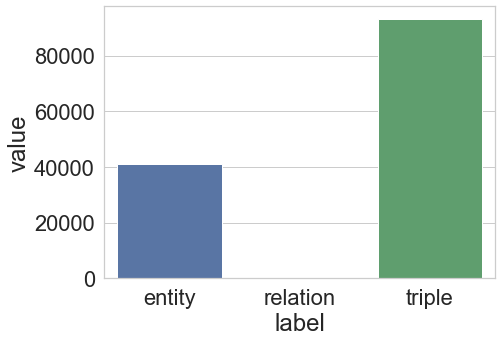
\includegraphics[width=0.45\textwidth]{WN18RR_Counts}
		\caption{WN18RR Property Barplot}
		}
	\hfill
	\parbox{.5\linewidth}{
   		\centering
    		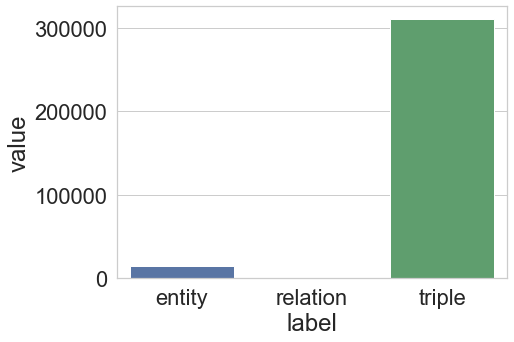
\includegraphics[width=0.45\textwidth]{FB15k-237_Counts}
		\caption{FB15k-237 Property Barplot}
		}
\end{figure}

\begin{table}[H]
	\parbox{.5\linewidth}{
		\centering
		\begin{tabular}{lllllllllll}
  			\textbf{Property} & \textbf{Count}  \\
  			\hline
  			Entities & 40,943  \\
  			Relations & 11  \\
  			Triples & 93,003 \\
			&
		\end{tabular}
		\caption{WN18RR Property Counts}
		}
	\hfill
	\parbox{.5\linewidth}{
		\centering
		\begin{tabular}{lllllllllll}
  			\textbf{Property} & \textbf{Count}  \\
  			\hline
  			Entities & 14,541   \\
  			Relations & 237  \\
  			Triples & 310,116  \\
			&
		\end{tabular}
		\caption{FB15k-237 Property Counts}
		}
\end{table}

%********************************** %Predicate **************************************

\noindent Summary statistics of the respective KG RDF formalism are presented below.

\begin{figure}[H]
	\parbox{.5\linewidth}{
   		\centering
    		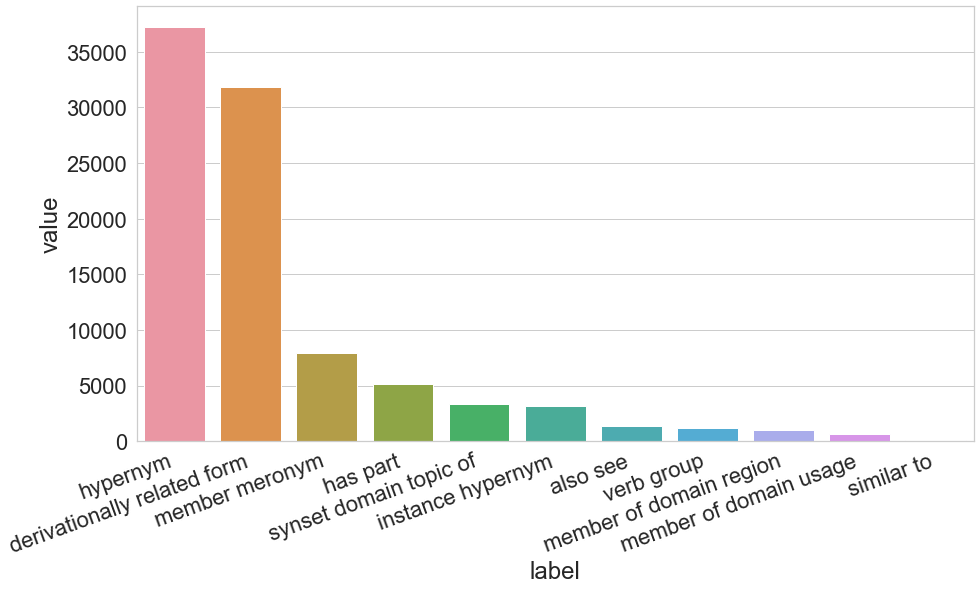
\includegraphics[width=0.45\textwidth, height=0.2\textheight]{WN18RR_Predicate_Counts}
		\caption{WN18RR Predicate Barplot}
		}
	\hfill
	\parbox{.5\linewidth}{
   		\centering
		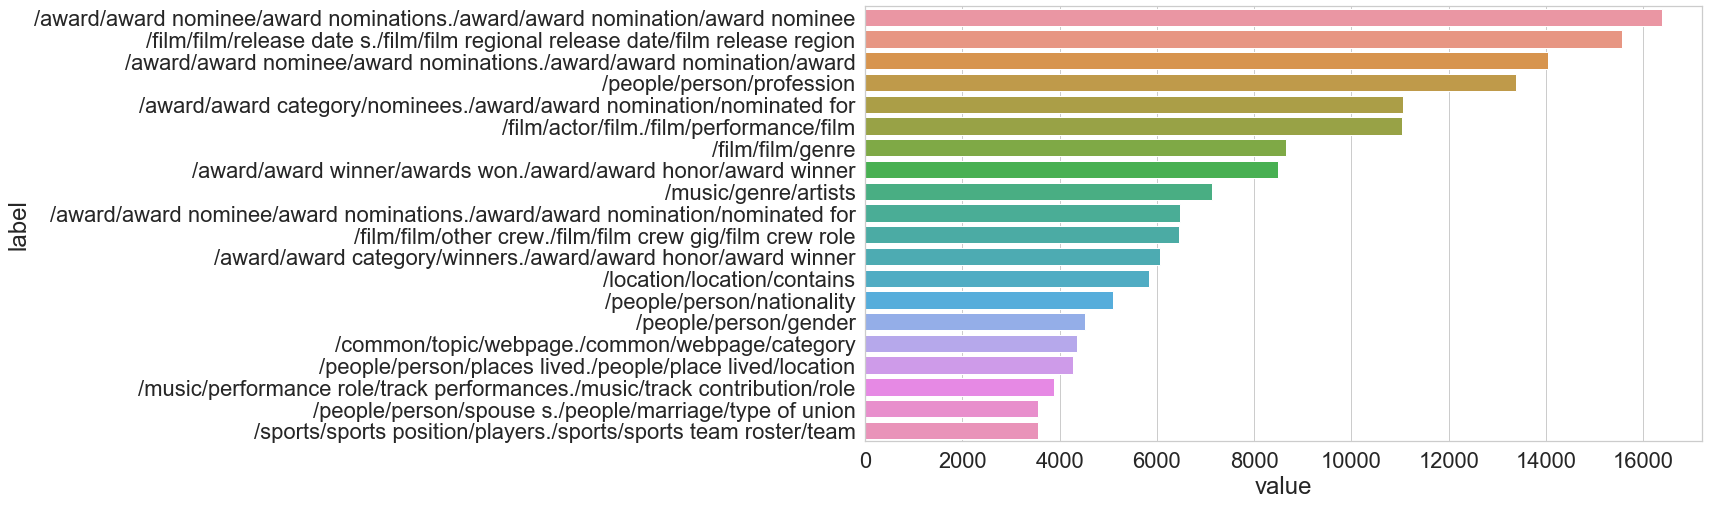
\includegraphics[width=0.45\textwidth, height=0.2\textheight]{FB15k-237_Predicate_Counts}
		\caption{FB15k-237 Predicate Barplot}
		}
\end{figure}

\begin{table}[H]
	\parbox{.5\linewidth}{
		\centering
		\begin{tabular}{lllllllllll}
  			\textbf{Statistic} & \textbf{Value}  \\
  			\hline
			Count & 11 \\
			Max & 37,221  \\
			Min & 86 \\
  			Median & 3150  \\
  			IQR & 5433.5  \\
			&
		\end{tabular}
		\caption{WN18RR Predicate Statistics}
		}
	\hfill
	\parbox{.5\linewidth}{
		\centering
		\begin{tabular}{lllllllllll}
  			\textbf{Statistic} & \textbf{Value}  \\
  			\hline
			Count & 237 \\
			Max & 16,391 \\
			Min & 45  \\
  			Median & 426  \\
  			IQR & 819 \\
			&
		\end{tabular}
		\caption{FB15k-237 Predicate Statistics}
		}
\end{table}

%********************************** %Subject **************************************

\begin{figure}[H]
	\parbox{.5\linewidth}{
   		\centering
    		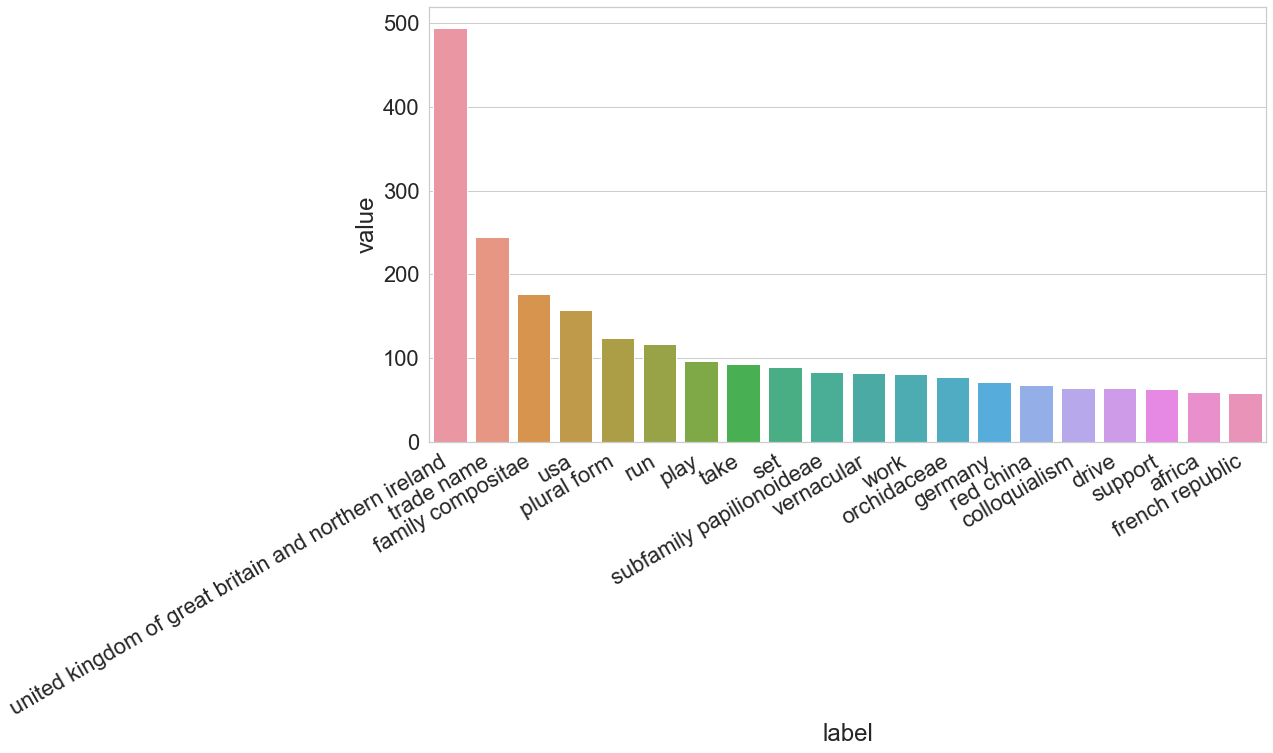
\includegraphics[width=0.45\textwidth, height=0.2\textheight]{WN18RR_Subject_Counts}
		\caption{WN18RR Subject Barplot}
		}
	\hfill
	\parbox{.5\linewidth}{
   		\centering
		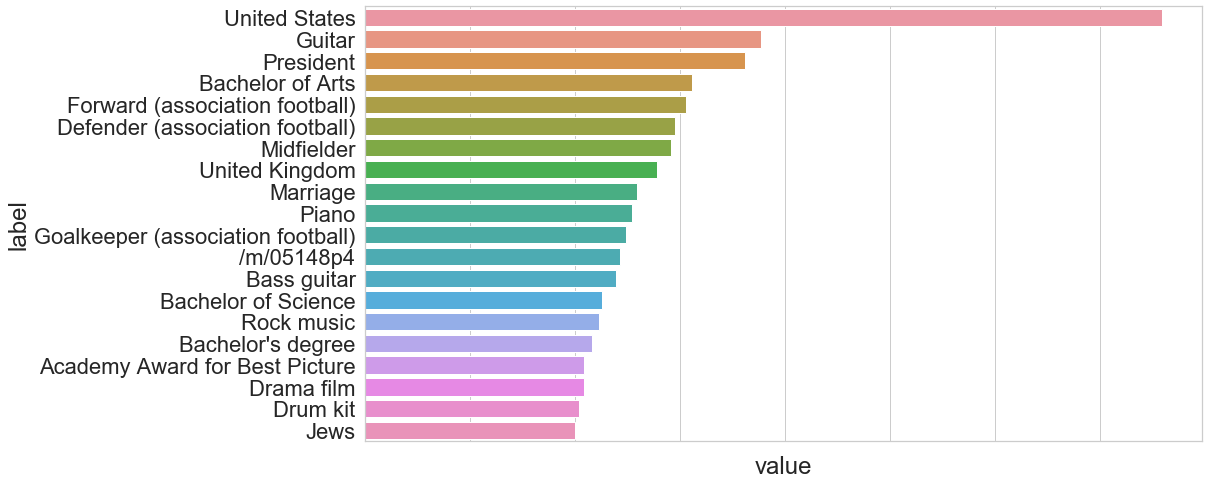
\includegraphics[width=0.45\textwidth, height=0.2\textheight]{FB15k-237_Subject_Counts}
		\caption{FB15k-237 Subject Barplot}
		}
\end{figure}

\begin{table}[H]
	\parbox{.5\linewidth}{
		\centering
		\begin{tabular}{lllllllllll}
  			\textbf{Statistic} & \textbf{Value}  \\
  			\hline
			Count & 32,349 \\
			Max & 494 \\
			Min & 1 \\
  			Median & 2 \\
  			IQR & 2 \\
			&
		\end{tabular}
		\caption{WN18RR Subject Statistics}
		}
	\hfill
	\parbox{.5\linewidth}{
		\centering
		\begin{tabular}{lllllllllll}
  			\textbf{Statistic} & \textbf{Value}  \\
  			\hline
			Count &13,891 \\
			Max & 1,518 \\
			Min & 1 \\
  			Median & 16 \\
  			IQR & 20 \\
			&
		\end{tabular}
		\caption{FB15k-237 Subject Statistics}
		}
\end{table}

%********************************** %Object **************************************

\begin{figure}[H]
	\parbox{.5\linewidth}{
   		\centering
    		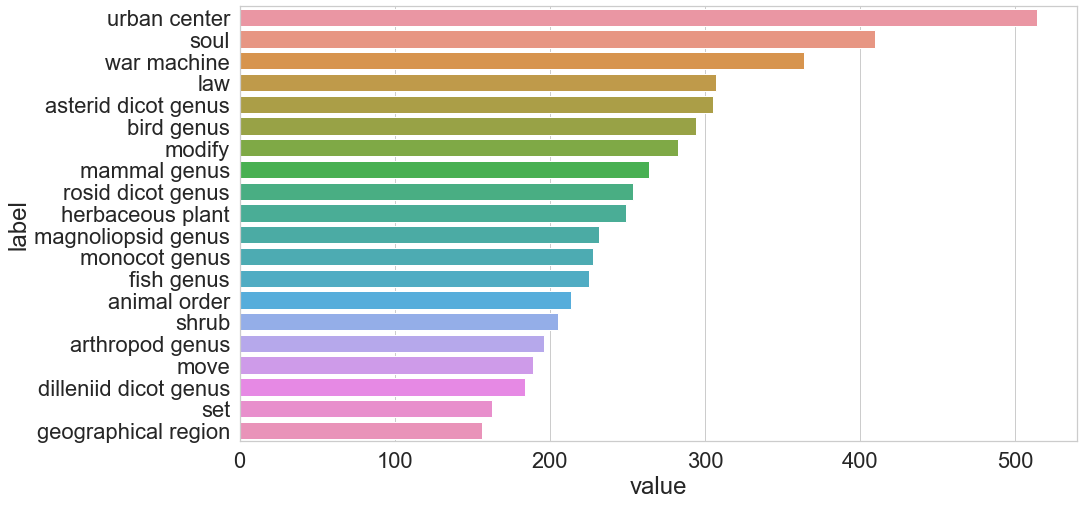
\includegraphics[width=0.45\textwidth, height=0.2\textheight]{WN18RR_Object_Counts}
		\caption{WN18RR Object Barplot}
		}
	\hfill
	\parbox{.5\linewidth}{
   		\centering
		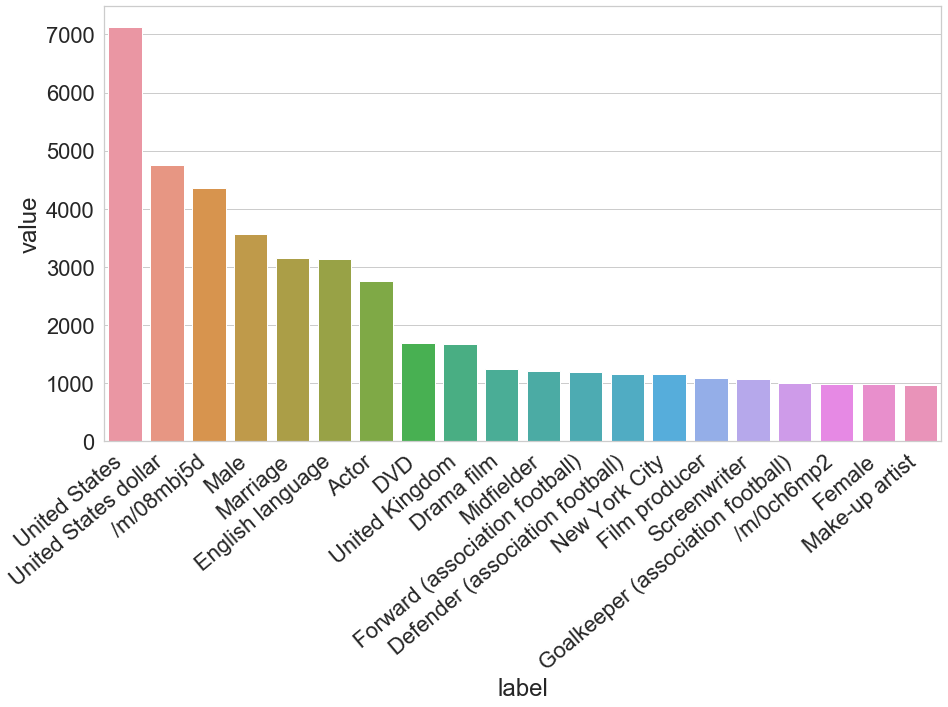
\includegraphics[width=0.45\textwidth, height=0.2\textheight]{FB15k-237_Object_Counts}
		\caption{FB15k-237 Object Barplot}
		}
\end{figure}


\begin{table}[H]
	\parbox{.5\linewidth}{
		\centering
		\begin{tabular}{lllllllllll}
  			\textbf{Statistic} & \textbf{Value}  \\
  			\hline
			Count & 26,162 \\
			Max & 514 \\
			Min & 1 \\
  			Median & 1 \\
  			IQR & 2 \\
			&
		\end{tabular}
		\caption{WN18RR Object Statistics}
		}
	\hfill
	\parbox{.5\linewidth}{
		\centering
		\begin{tabular}{lllllllllll}
  			\textbf{Statistic} & \textbf{Value}  \\
  			\hline
			Count & 13,504 \\
			Max & 7,124 \\
			Min & 1 \\
  			Median & 10 \\
  			IQR & 16 \\
			&
		\end{tabular}
		\caption{FB15k-237 Object Statistics}
		}
\end{table}

\noindent For WN18RR, it can be seen that relations are skewed toward the relations "hypernym" and "derivationally related from", with a maximum of 37,221 occurrences, with an IQR of 5433.5 and 819 respectively. FB15k-237 are skewed toward film relations. We would expect reasonable performance across this type of relation for the knowledge graph. WN18R and FB15k-237 subjects are somewhat uniform aside from a small number of high occurrences entities, with the median number of occurrences is 3 and 16 respectively, and with an IQR of 2 and 20 respectively. WN18RR object occurrences are somewhat uniform. FB15k-237 object occurrences are skewed, with the "United States" partaking in the highest number of facts. This is in comparison to a median object occurrence of 1 and an interquartile range of 10,
and an IQR of 2 and 16 respectively. Such high variance in FB15k-237 suggests poor potential model performance for FB15k-237 relative to WN18RR. 


%********************************** %Pre-Trained Word Embeddings **************************************

\subsection{HypER+ with glove word embeddings}

HypER+ here is implemented using Glove pre-trained word embeddings. The the model was trained on Google Cloud Platform, on a N1 series instance with  8 CPU cores, 30GB RAM, 512GB SSD and a Nvidia Tesla P100 GPU. We evaluate the model using standard link prediction benchmarks. \par 

\noindent \textbf{Code to reproduce} \newline
HypER+ with GloVe: \url{https://github.com/xhosaBoy/HypER-Pretrained-Word-Vectors} \newline
Baseline: \url{https://github.com/xhosaBoy/HypER-baseline} 

\noindent {Link prediction results.} The link prediction benchmark results of the HypER+ with pre-trained embeddings model, compared against other link prediction models, are presented below.

%********************************** %Cost **************************************

\begin{figure}[H]
	\parbox{.5\linewidth}{
   		\centering
    		\includegraphics[width=0.45\textwidth, height=0.2\textheight]{WN18RR_Cost_Results}
		\caption{WN18RR Cost}
		}
	\hfill
	\parbox{.5\linewidth}{
   		\centering
		\includegraphics[width=0.45\textwidth, height=0.2\textheight]{FB15k-237_Cost_Results}
		\caption{FB15k-237 Cost}
		}
\end{figure}

%********************************** %Hits@10 **************************************

\begin{figure}[H]
	\parbox{.5\linewidth}{
   		\centering
    		\includegraphics[width=0.45\textwidth, height=0.2\textheight]{WN18RR_hits_at_10_Results}
		\caption{WN18RR Hits@10}
		}
	\hfill
	\parbox{.5\linewidth}{
   		\centering
		\includegraphics[width=0.45\textwidth, height=0.2\textheight]{FB15k-237_hits_at_10_Results}
		\caption{FB15k-237 Hits@10}
		}
\end{figure}

%********************************** %Hits@3 **************************************

\begin{figure}[H]
	\parbox{.5\linewidth}{
   		\centering
    		\includegraphics[width=0.45\textwidth, height=0.2\textheight]{WN18RR_hits_at_3_Results}
		\caption{WN18RR Hits@3}
		}
	\hfill
	\parbox{.5\linewidth}{
   		\centering
		\includegraphics[width=0.45\textwidth, height=0.2\textheight]{FB15k-237_hits_at_3_Results}
		\caption{FB15k-237 Hits@3}
		}
\end{figure}

%********************************** %Hits@1 **************************************

\begin{figure}[H]
	\parbox{.5\linewidth}{
   		\centering
    		\includegraphics[width=0.45\textwidth, height=0.2\textheight]{WN18RR_hits_at_1_Results}
		\caption{WN18RR Hits@1}
		}
	\hfill
	\parbox{.5\linewidth}{
   		\centering
		\includegraphics[width=0.45\textwidth, height=0.2\textheight]{FB15k-237_hits_at_1_Results}
		\caption{FB15k-237 Hits@1}
		}
\end{figure}

%********************************** %Mean rank **************************************

\begin{figure}[H]
	\parbox{.5\linewidth}{
   		\centering
    		\includegraphics[width=0.45\textwidth, height=0.2\textheight]{WN18RR_mean_rank_Results}
		\caption{WN18RR Mean Rank}
		}
	\hfill
	\parbox{.5\linewidth}{
   		\centering
		\includegraphics[width=0.45\textwidth, height=0.2\textheight]{FB15k-237_mean_rank_Results}
		\caption{FB15k-237 Mean Rank}
		}
\end{figure}

%********************************** %Mean reciprocal rank **************************************

\begin{figure}[H]
	\parbox{.5\linewidth}{
   		\centering
    		\includegraphics[width=0.45\textwidth, height=0.2\textheight]{WN18RR_mean_reciprocal_rank_Results}
		\caption{WN18RR Mean Reciprocal Rank}
		}
	\hfill
	\parbox{.5\linewidth}{
   		\centering
		\includegraphics[width=0.45\textwidth, height=0.2\textheight]{FB15k-237_mean_reciprocal_rank_Results}
		\caption{FB15k-237 Mean Reciprocal Rank}
		}
\end{figure}

%********************************** %Test results **************************************

\begin{table}[H]
	\parbox{.5\linewidth}{
		\centering
		\resizebox{0.5\columnwidth}{!}{
		\begin{tabular}{lllllllllll}
  			\textbf{Model} & \textbf{H@10} & \textbf{H@3} & \textbf{H@1} & \textbf{MR} & \textbf{MRR} \\
  			\hline
  			DistMult (Yang et al. 2015) & .490 & .440 & .390 & 5110 & .430 \\
  			ComplEx (Trouillon et al. 2016) & .510 & .460 & .410 & 5261 & .440 \\
  			Neural LP (Yang, Yang, and Cohen 2017) & - & - & - & - & - \\
			MINERVA (Das et al. 2018) & - & - & - & - & - \\
			ConvE (Dettmers et al. 2018) & .520 & .440 & .400 & 4187 & .430 \\
			HypER (Bala\v{z}evi\'c et al. 2019) & .522 & .477 & \textbf{.436} & 5798 & .465 \\
  			\hline
  			HypER+ (ours) & \textbf{.552} & \textbf{.481} & .432 & \textbf{1586} & \textbf{.471} \\
			&
		\end{tabular}
		}
		\captionsetup{justification=centering}
		\caption{Test results on WN18RR}
	}
	\hfill
	\parbox{.5\linewidth}{
		\centering
		\resizebox{0.5\columnwidth}{!}{
		\begin{tabular}{lllllllllll}
  			\textbf{Model} & \textbf{H@10} & \textbf{H@3} & \textbf{H@1} & \textbf{MR} & \textbf{MRR} \\
  			\hline
  			DistMult (Yang et al. 2015) & .419 & .263 & .155 & 254 & .241 \\
  			ComplEx (Trouillon et al. 2016) & .428 & .275 & .158 & 339 & .247 \\
  			Neural LP (Yang, Yang, and Cohen 2017) & .408 & - & - & - & .250 \\
			MINERVA (Das et al. 2018) & .456 & - & - & - & - \\
			ConvE (Dettmers et al. 2018) & .501 & .356 & .237 & 244 & .325 \\
			HypER (Bala\v{z}evi\'c et al. 2019) & .520 & \textbf{.376} & \textbf{.252} & 250 & \textbf{.341} \\
  			\hline
  			HypER+ (ours) & \textbf{.522} & \textbf{.376} & \textbf{.252} & \textbf{215} & \textbf{.341} \\
			&
		\end{tabular}
		}
		\captionsetup{justification=centering}
		\caption{Test results on FB15k-237}
	}
\end{table}

%********************************** %Test Result Decomposition **************************************

\begin{table}[H]
	\centering
	\resizebox{0.5\columnwidth}{!}{
	\begin{tabular}{lllllllllll}
  		\textbf{Subject} & \textbf{Predicate} & \textbf{Object Target} & \textbf{Object Prediction} \\
  		\hline
  		usa & has part & colorado & missouri river \\
  		spain & has part & cadiz & jerez de la frontera \\
  		kilobyte & has part & computer memory unit & word \\
		electromagnetic spectrum & has part & actinic ray & radio spectrum \\
		systema respiratorium & has part & respiratory tract & respiratory organ \\
		respiratory organ & has part & nsa & defense advanced research projects agency \\
		africa & has part & nigeria & senegal \\
  		antigen & has part & substance & epitope \\
		amphitheatre & has part & theatre & tiered seat \\
		indian ocean & has part & mauritius & antarctic ocean \\
		&
	\end{tabular}
	}
	\caption{Qualitative Hit@1 Test results on WN18RR}
\end{table}

\begin{figure}[H]
   	\centering
    	\includegraphics[width=0.5\textwidth, height=0.2\textheight]{WN18RR_relational_performance_results}
	\captionsetup{justification=centering}
	\caption{WN18RR Hit@ 1 Predicate Performance}
\end{figure}


%********************************** %Chapter Summary  **************************************

\section{Summary}

\textbf{NTN with optimised training algorithm.} We've attempted a simple improvement in the NTN model by appplying modern deep learning training techniques, including Adam and hyperparameter random search. The results indicate there potential performance gains by deep models simply by updating their respective training algorithms with modern methods. In this instance, we see an accuracy gain of 6.2\%, for the Wordnet and Freebase datasets. \newline
\noindent \textbf{HypER+.}  Here we compensate for the covariate shift introduced by the hypernetwork in convolutional factorisation. The distributional drift is pronounced enough that we are able to improve the Hit@1 accuracy on of the original HypER model on average by 2.7\%, for the WN18 and FB15k datasets.\newline
\noindent \textbf{HypER+ with GloVe.} Finally we extend HypER+ to make use of pre-trained GloVe word vectors. The semantic information inherent in these embeddings somewhat overpower the structural information present in the knowledge graph. The resultant model on average decreases the Hit@1 accuracy on of the original HypER model on average by 0.4\%, for the WN18RR and FB15k-237 datasets. \newline
